\documentclass[conference]{IEEEtran}

\usepackage[utf8]{inputenc}
\usepackage[T1]{fontenc}
\usepackage[spanish,es-tabla]{babel}

\usepackage{amsmath,amssymb}
\usepackage{graphicx}
\graphicspath{{prism-uploads/}}
\usepackage{booktabs}
\usepackage{array}
\usepackage{url}
\usepackage{cite}
\usepackage{multirow}
\usepackage{xcolor}

\title{Predicción de la Localización de Personas Desaparecidas en Ecuador mediante Redes Neuronales MLP Optimizadas Comparativamente con Algoritmos Genéticos y Enjambre de Partículas}

\author{
\begin{tabular}{cc}
\begin{minipage}{0.46\textwidth}
\centering
Luis Gonzalo Ordóñez Yaguana\\
\textit{Carrera de Ciencia de Datos e IA}\\
\textit{Universidad Nacional de Chimborazo}\\
\textit{Riobamba, Ecuador}\\
gonzalo.ordonez@unach.edu.ec\\
ORCID: 0009-0009-7864-837X
\end{minipage}
&
\begin{minipage}{0.46\textwidth}
\centering
Marcus Alexander Mayorga Martínez\\
\textit{Carrera de Ciencia de Datos e IA}\\
\textit{Universidad Nacional de Chimborazo}\\
\textit{Riobamba, Ecuador}\\
marcus.mayorga@unach.edu.ec\\
ORCID: 0009-0006-6916-9447
\end{minipage}
\\[4.0em]
\begin{minipage}{0.46\textwidth}
\centering
Jhoffre Marcelo Moreano Goyes\\
\textit{Carrera de Ciencia de Datos e IA}\\
\textit{Universidad Nacional de Chimborazo}\\
\textit{Riobamba, Ecuador}\\
jhoffre.moreano@unach.edu.ec\\
ORCID: 0009-0007-1521-4043
\end{minipage}
&
\begin{minipage}{0.46\textwidth}
\centering
Juan Sebastián Caviedes Rodríguez\\
\textit{Carrera de Ciencia de Datos e IA}\\
\textit{Universidad Nacional de Chimborazo}\\
\textit{Riobamba, Ecuador}\\
juan.caviedes@unach.edu.ec\\
ORCID: 0009-0009-5098-892X
\end{minipage}
\end{tabular}
}

\begin{document}
\raggedbottom
\maketitle

\begin{abstract}
La desaparición de personas constituye un problema social y operativo crítico que exige mecanismos de análisis oportunos y rigurosos. Este artículo documenta el desarrollo de un sistema predictivo para estimar la probabilidad de localización exitosa de personas desaparecidas en Ecuador durante el periodo 2017--2025. Se comparan dos metodologías híbridas basadas en metaheurísticas poblacionales: un perceptrón multicapa (MLP) optimizado mediante un algoritmo genético (GA) y otro optimizado mediante enjambre de partículas (PSO). Ambas metaheurísticas exploran automáticamente la arquitectura de la red y sus hiperparámetros, incluida la regularización L2 y el \textit{dropout}. El flujo de trabajo incorpora control de fuga de información, \textit{target encoding} suavizado para categorías geográficas de alta cardinalidad, selección de variables por consenso y pesos de clase para abordar el desbalanceo (93.18\% de localizaciones exitosas). En el conjunto de prueba independiente, el MLP base obtuvo la mayor exactitud (90.78\%) y la menor latencia de inferencia (0.0519 ms). La variante MLP + GA alcanzó el mayor F1 macro (0.6745) y el menor \textit{log loss} (0.4692), mientras que MLP + PSO registró 90.17\% de exactitud y el menor tiempo de entrenamiento (98.74 s). La explicabilidad local y global se abordó mediante SHAP y LIME para aportar trazabilidad a las predicciones.
\end{abstract}

\begin{IEEEkeywords}
personas desaparecidas, perceptrón multicapa, algoritmo genético, enjambre de partículas, regularización L2, pesos de clase, explicabilidad, SHAP, LIME.
\end{IEEEkeywords}

\section{Introducción}
La desaparición de personas representa una problemática social prioritaria en Ecuador. La capacidad de las instituciones de seguridad para evaluar oportunamente el riesgo asociado a un reporte depende, en gran medida, del procesamiento adecuado de la información demográfica y geográfica disponible al momento de la denuncia \cite{biehal2003lost,phoenix2022police,sidebottom2025can,tansill2026when}. Dado que cerca del 93\% de las desapariciones concluyen en localizaciones exitosas, la identificación del pequeño porcentaje de casos complejos constituye el principal reto analítico.

Los datos históricos recopilados por la Fiscalía General del Estado (FGE) y la Policía Nacional presentan un marcado desbalanceo de clases y riesgos de fuga de información (\textit{data leakage}). La predicción de eventos raros o desbalanceados se ha abordado mediante algoritmos de aprendizaje supervisado en ámbitos sociales y de salud \cite{ruizrizzo2022predicting}. Evitar la fuga de datos es indispensable para evaluar los clasificadores de forma realista en el ``día cero'' de la denuncia.

Este artículo propone y contrasta dos metaheurísticas bioinspiradas para ajustar los hiperparámetros de redes neuronales densas: un algoritmo genético y la optimización por enjambre de partículas. Ambas estrategias realizan una búsqueda global sobre un espacio combinatorio que incluye regularización L2 (\textit{weight decay}) para controlar la complejidad del modelo. El sistema resultante integra las inferencias con técnicas de inteligencia artificial explicable (XAI), específicamente SHAP y LIME, en una interfaz interactiva desarrollada con Streamlit.

\section{Metodología}
El flujo metodológico comprende extracción, transformación y carga (ETL), selección de características por consenso, ajuste de hiperparámetros, validación estadística y explicabilidad local y global. Este proceso toma como referencia trabajos recientes de analítica de datos aplicados al contexto ecuatoriano \cite{espinoza2025predictive,quinga2025data}.

\begin{figure}[!t]
\centering
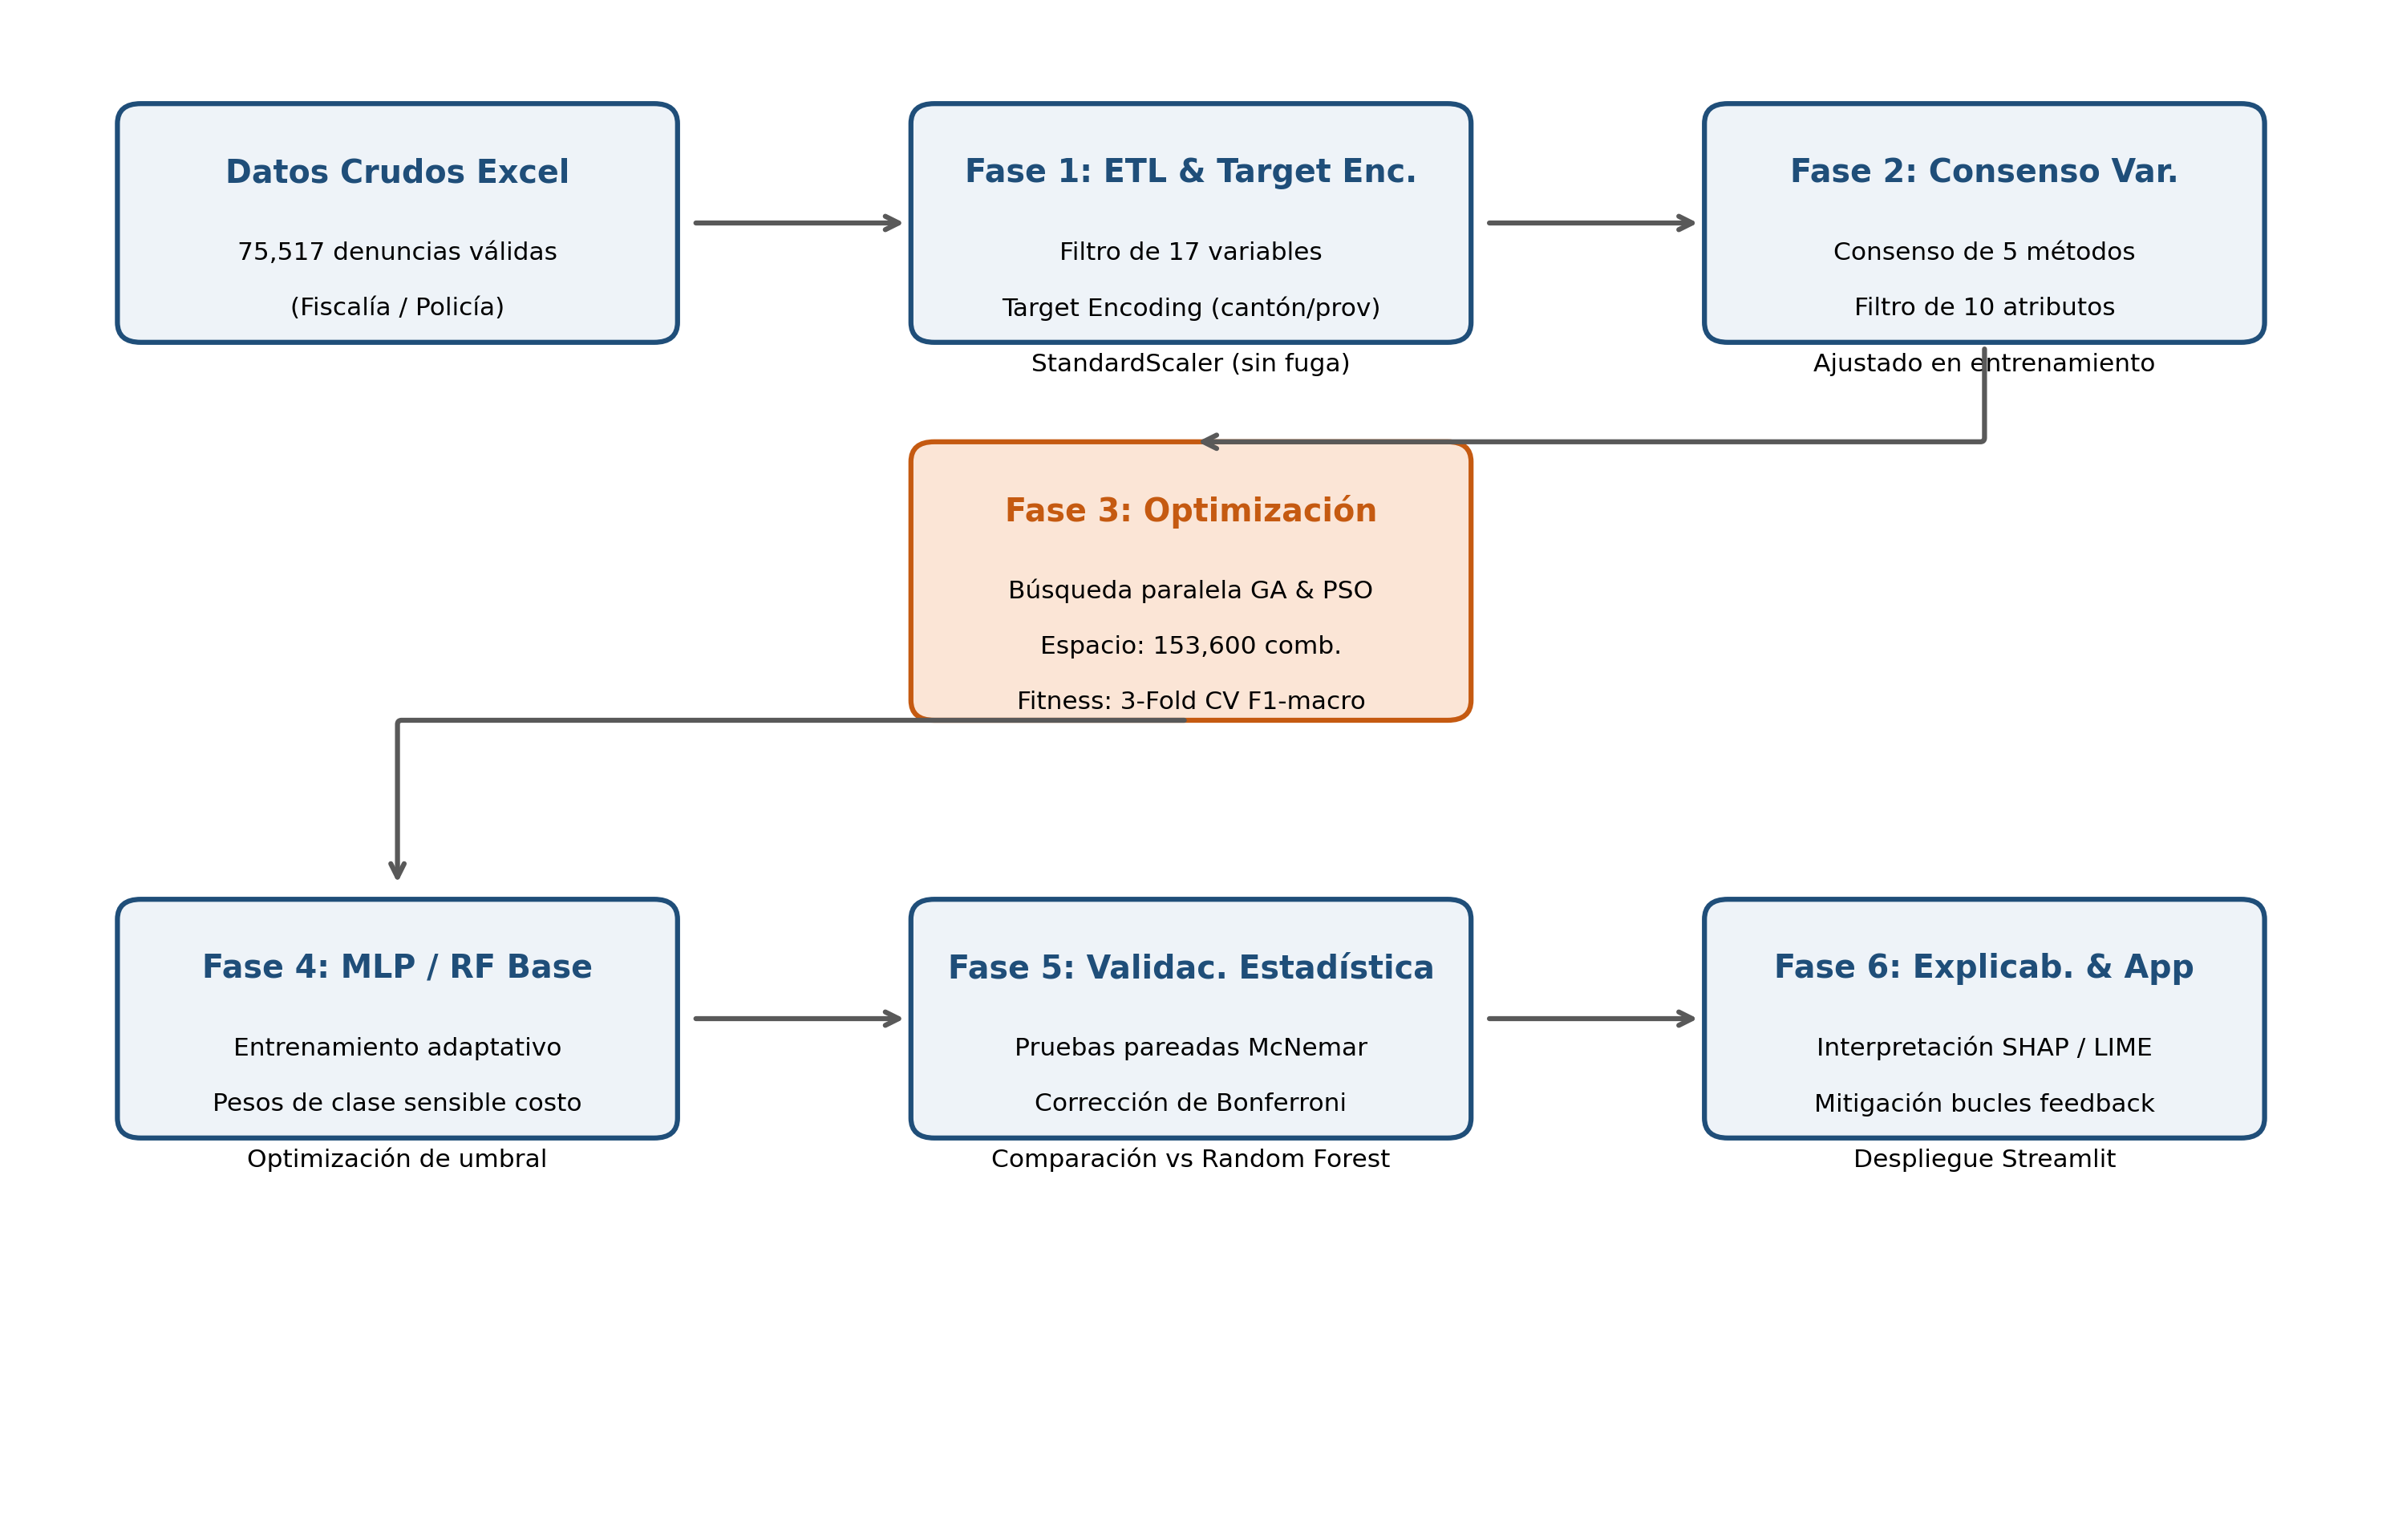
\includegraphics[width=\linewidth]{image.png}
\caption{Esquema resumido del flujo de procesamiento, desde el conjunto de datos original hasta el entrenamiento y despliegue del modelo.}
\label{fig:pipeline}
\end{figure}

\begin{figure}[!t]
\centering
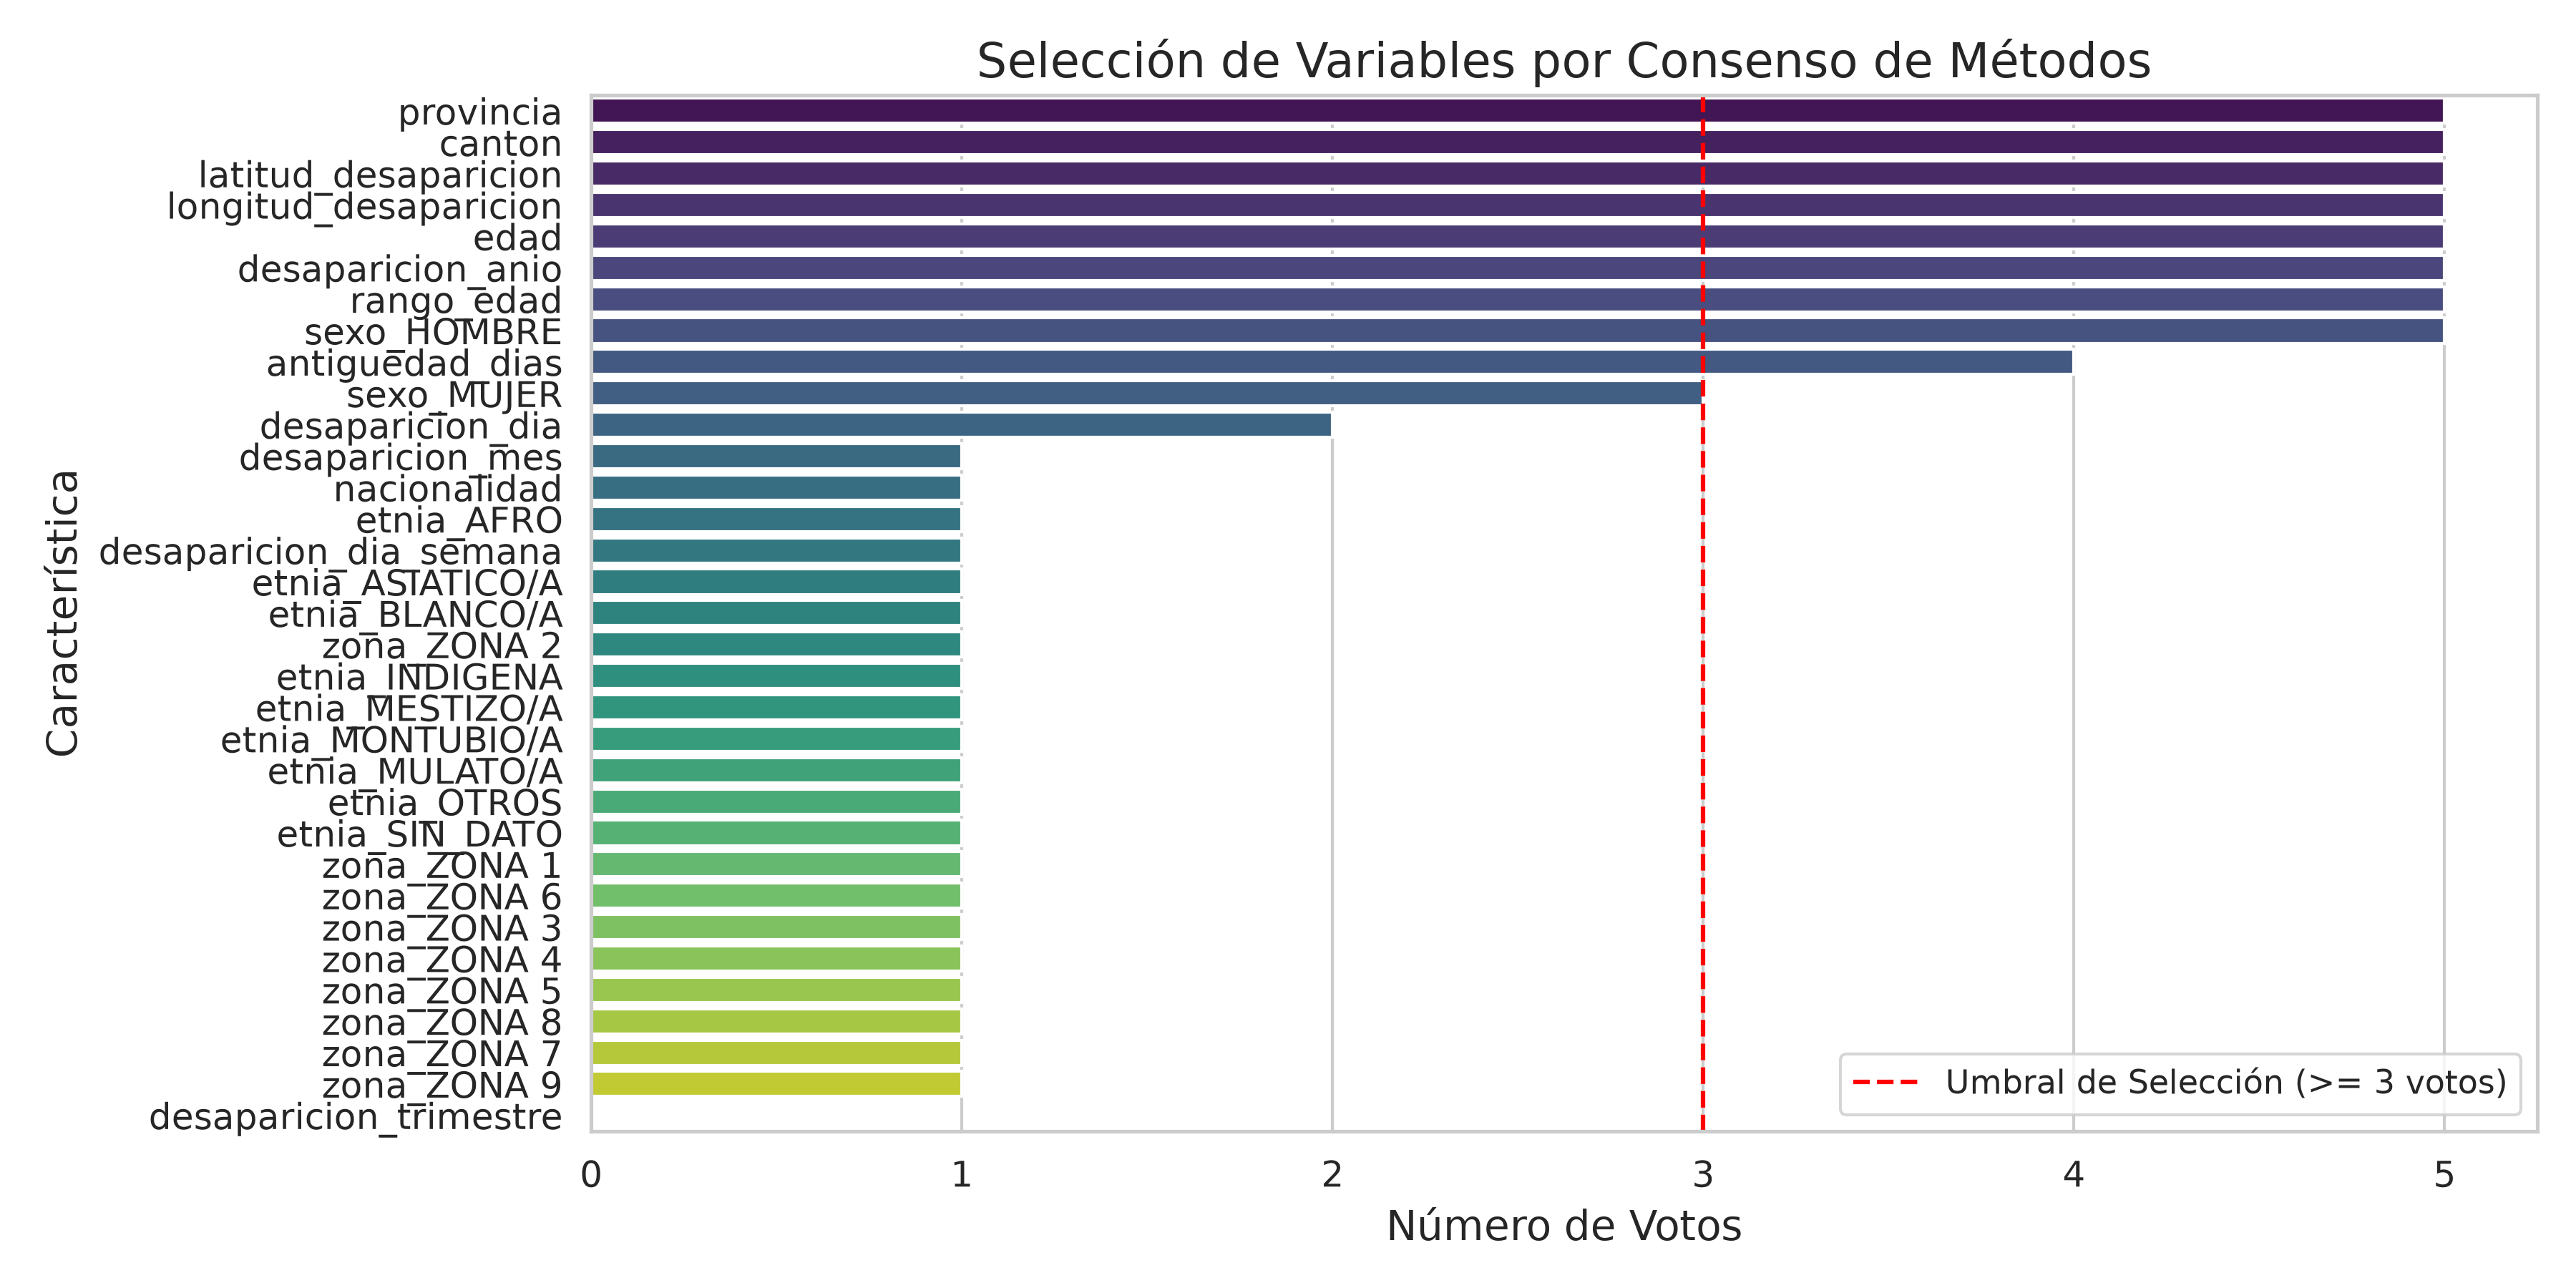
\includegraphics[width=0.95\linewidth]{12_seleccion_consenso.png}
\caption{Selección de las diez características principales mediante consenso de cinco métodos: correlación de Pearson, importancia por permutación, SHAP, RFE e información mutua.}
\label{fig:consenso}
\end{figure}

\subsection{Fase 1: ETL y Codificación de Alta Cardinalidad}
A partir del conjunto consolidado de 75,680 registros oficiales (2017--2025), se depuraron coordenadas espaciales nulas e inconsistencias temporales. Se eliminaron 17 columnas causantes de fuga de datos, como los días transcurridos hasta la solución o la provincia de localización, para evitar sobreestimaciones artificiales del desempeño predictivo \cite{kaufman2012leakage}. Las variables espaciales de alta cardinalidad, como cantón y provincia, se transformaron mediante \textit{target encoding} regularizado con suavizado para reducir el riesgo de sobreajuste.

\subsection{Fase 2: Selección de Características por Consenso}
Se ejecutó un proceso de selección por consenso de cinco métodos: correlación de Pearson, importancia por permutación, contribuciones de Shapley (SHAP), eliminación recursiva de características (RFE) e información mutua. Este proceso determinó un vector final de diez atributos con alta relevancia predictiva (Fig. \ref{fig:consenso}), entre ellos cantón, provincia, coordenadas geográficas, edad y variables temporales.

\begin{figure}[htbp]
\centering
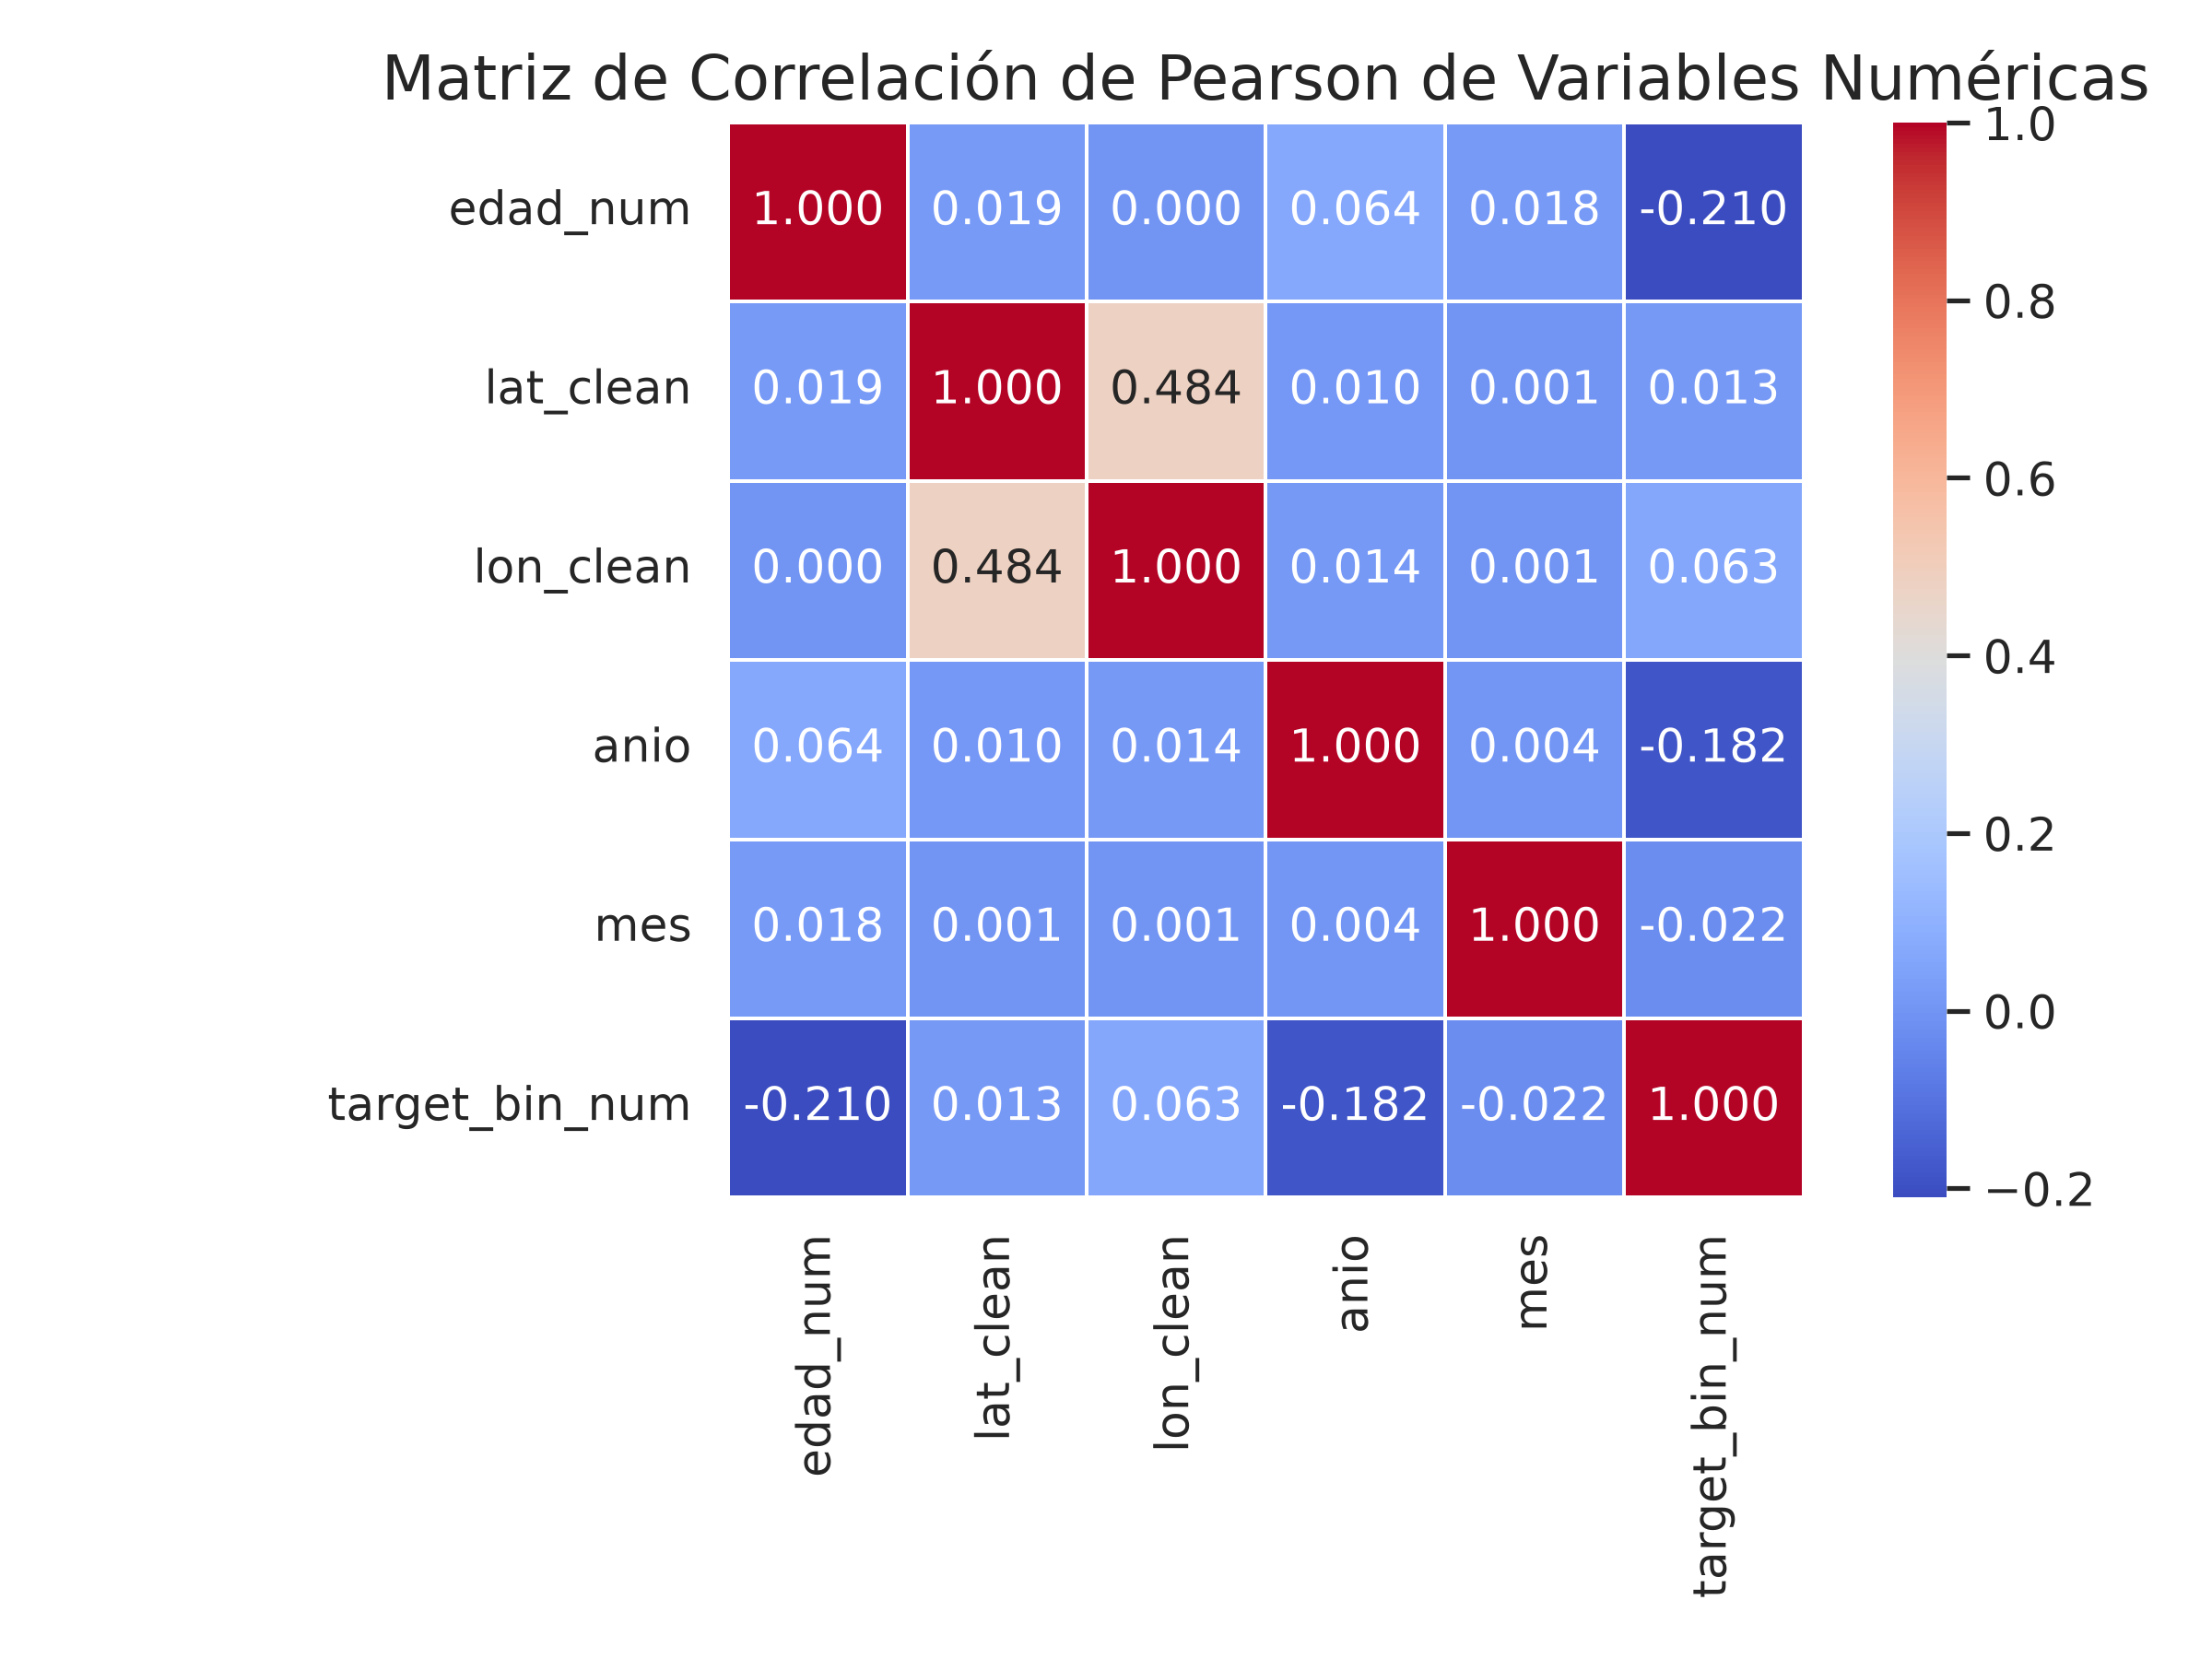
\includegraphics[width=0.95\linewidth]{09_matriz_correlacion.png}
\caption{Matriz de correlación de las variables numéricas empleadas durante el análisis exploratorio y la selección de características.}
\label{fig:correlacion}
\end{figure}

\subsection{Fase 3: Optimización Metaheurística}
Para ajustar automáticamente las redes MLP, se definió un espacio de búsqueda combinatorio compuesto por la tasa de aprendizaje, el número de capas ocultas, la cantidad de neuronas, el \textit{dropout}, el tamaño de lote, las funciones de activación, los optimizadores y el coeficiente de regularización L2. Como función de aptitud (\textit{fitness}) para guiar a ambos optimizadores, se utilizó el F1-Score macro obtenido mediante validación cruzada estratificada de 3 pliegues. Las metaheurísticas exploraron este espacio de la siguiente manera:
\begin{itemize}
    \item \textbf{Algoritmo genético (MLP + GA):} Implementado con la biblioteca DEAP mediante selección por torneo ($k=3$), cruce uniforme ($p_x=0.7$), mutación uniforme indexada ($p_m=0.2$) y preservación elitista.
    \item \textbf{Enjambre de Partículas (MLP + PSO):} Implementado mediante la dinámica de inercia lineal decreciente (\textit{Linear Inertia Weight Reduction - LIWR}), variando el peso de inercia $w_t$ desde $0.9$ hasta $0.4$ para transicionar de exploración global a explotación local fina.
\end{itemize}

\subsection{Fase 4: Entrenamiento e Inferencia Adaptativa}
Con las arquitecturas e hiperparámetros seleccionados, se entrenaron los modelos definitivos. El desbalanceo de clases (93.18\% de casos favorables y 6.82\% de casos desfavorables) se abordó mediante pesos de clase en la entropía cruzada binaria. Esta estrategia se prefirió frente a métodos de remuestreo sintético, como SMOTE, porque conserva la integridad espacial de los registros originales. Además, se realizó un barrido de umbrales entre 0.20 y 0.80, con incrementos de 0.01, para seleccionar el umbral de decisión que maximiza el F1 macro de cada clasificador.

\subsection{Fase 5: Validación Estadística}
Para determinar si las diferencias entre los clasificadores eran estadísticamente significativas, se aplicó la prueba de McNemar. Esta prueba utiliza una tabla de contingencia de dimensión $2\times2$ que reúne los resultados discordantes de dos modelos evaluados sobre el mismo conjunto de prueba:
\begin{equation}
\chi^2 = \frac{(|f_{12} - f_{21}| - 1)^2}{f_{12} + f_{21}}
\label{eq:mcnemar}
\end{equation}
donde $f_{12}$ representa las muestras en las que el primer modelo acierta y el segundo falla, mientras que $f_{21}$ representa el caso contrario. La expresión incorpora la corrección de continuidad de Yates.

\subsection{Fase 6: Explicabilidad (XAI) y Despliegue}
Para mejorar la transparencia operativa y reducir el carácter de ``caja negra'' de los modelos neuronales, se integraron dos niveles de explicabilidad:
\begin{itemize}
    \item \textbf{SHAP (explicación global):} Basado en valores de Shapley \cite{lundberg2017unified}, estima la contribución general de cada característica en el conjunto de datos.
    \item \textbf{LIME (explicación local):} Genera aproximaciones lineales interpretables alrededor de cada observación \cite{ribeiro2016why} para justificar visualmente las predicciones presentadas en la aplicación Streamlit.
\end{itemize}

\section{Configuración Experimental}
La Tabla \ref{tab:config-red} detalla las arquitecturas e hiperparámetros óptimos resultantes de la sintonización automática en comparación con la línea base manual.

\begin{table}[htbp]
\caption{Parámetros de las redes neuronales entrenadas}
\label{tab:config-red}
\centering
\setlength{\tabcolsep}{1.5pt}
\begin{tabular}{lccc}
\toprule
\textbf{Parámetro} & \textbf{MLP base} & \textbf{MLP + GA} & \textbf{MLP + PSO} \\
\midrule
Capas ocultas & 2 & 3 & 4 \\
Neuronas & 128 & 256 & 128 \\
Activación & ReLU / Sigmoide & ReLU / Sigmoide & ReLU / Sigmoide \\
Tasa de aprendizaje & 0.001 & 0.0005 & 0.0005 \\
\textit{Dropout} & 0.3 & 0.0 & 0.0 \\
Regularización L2 & Ninguna & 0.0001 & Ninguna \\
Tamaño de lote & 128 & 32 & 128 \\
Optimizador & Adam & RMSprop & Adam \\
Épocas & 30 & 30 & 100 \\
\bottomrule
\end{tabular}
\end{table}

\begin{figure}[htbp]
\centering
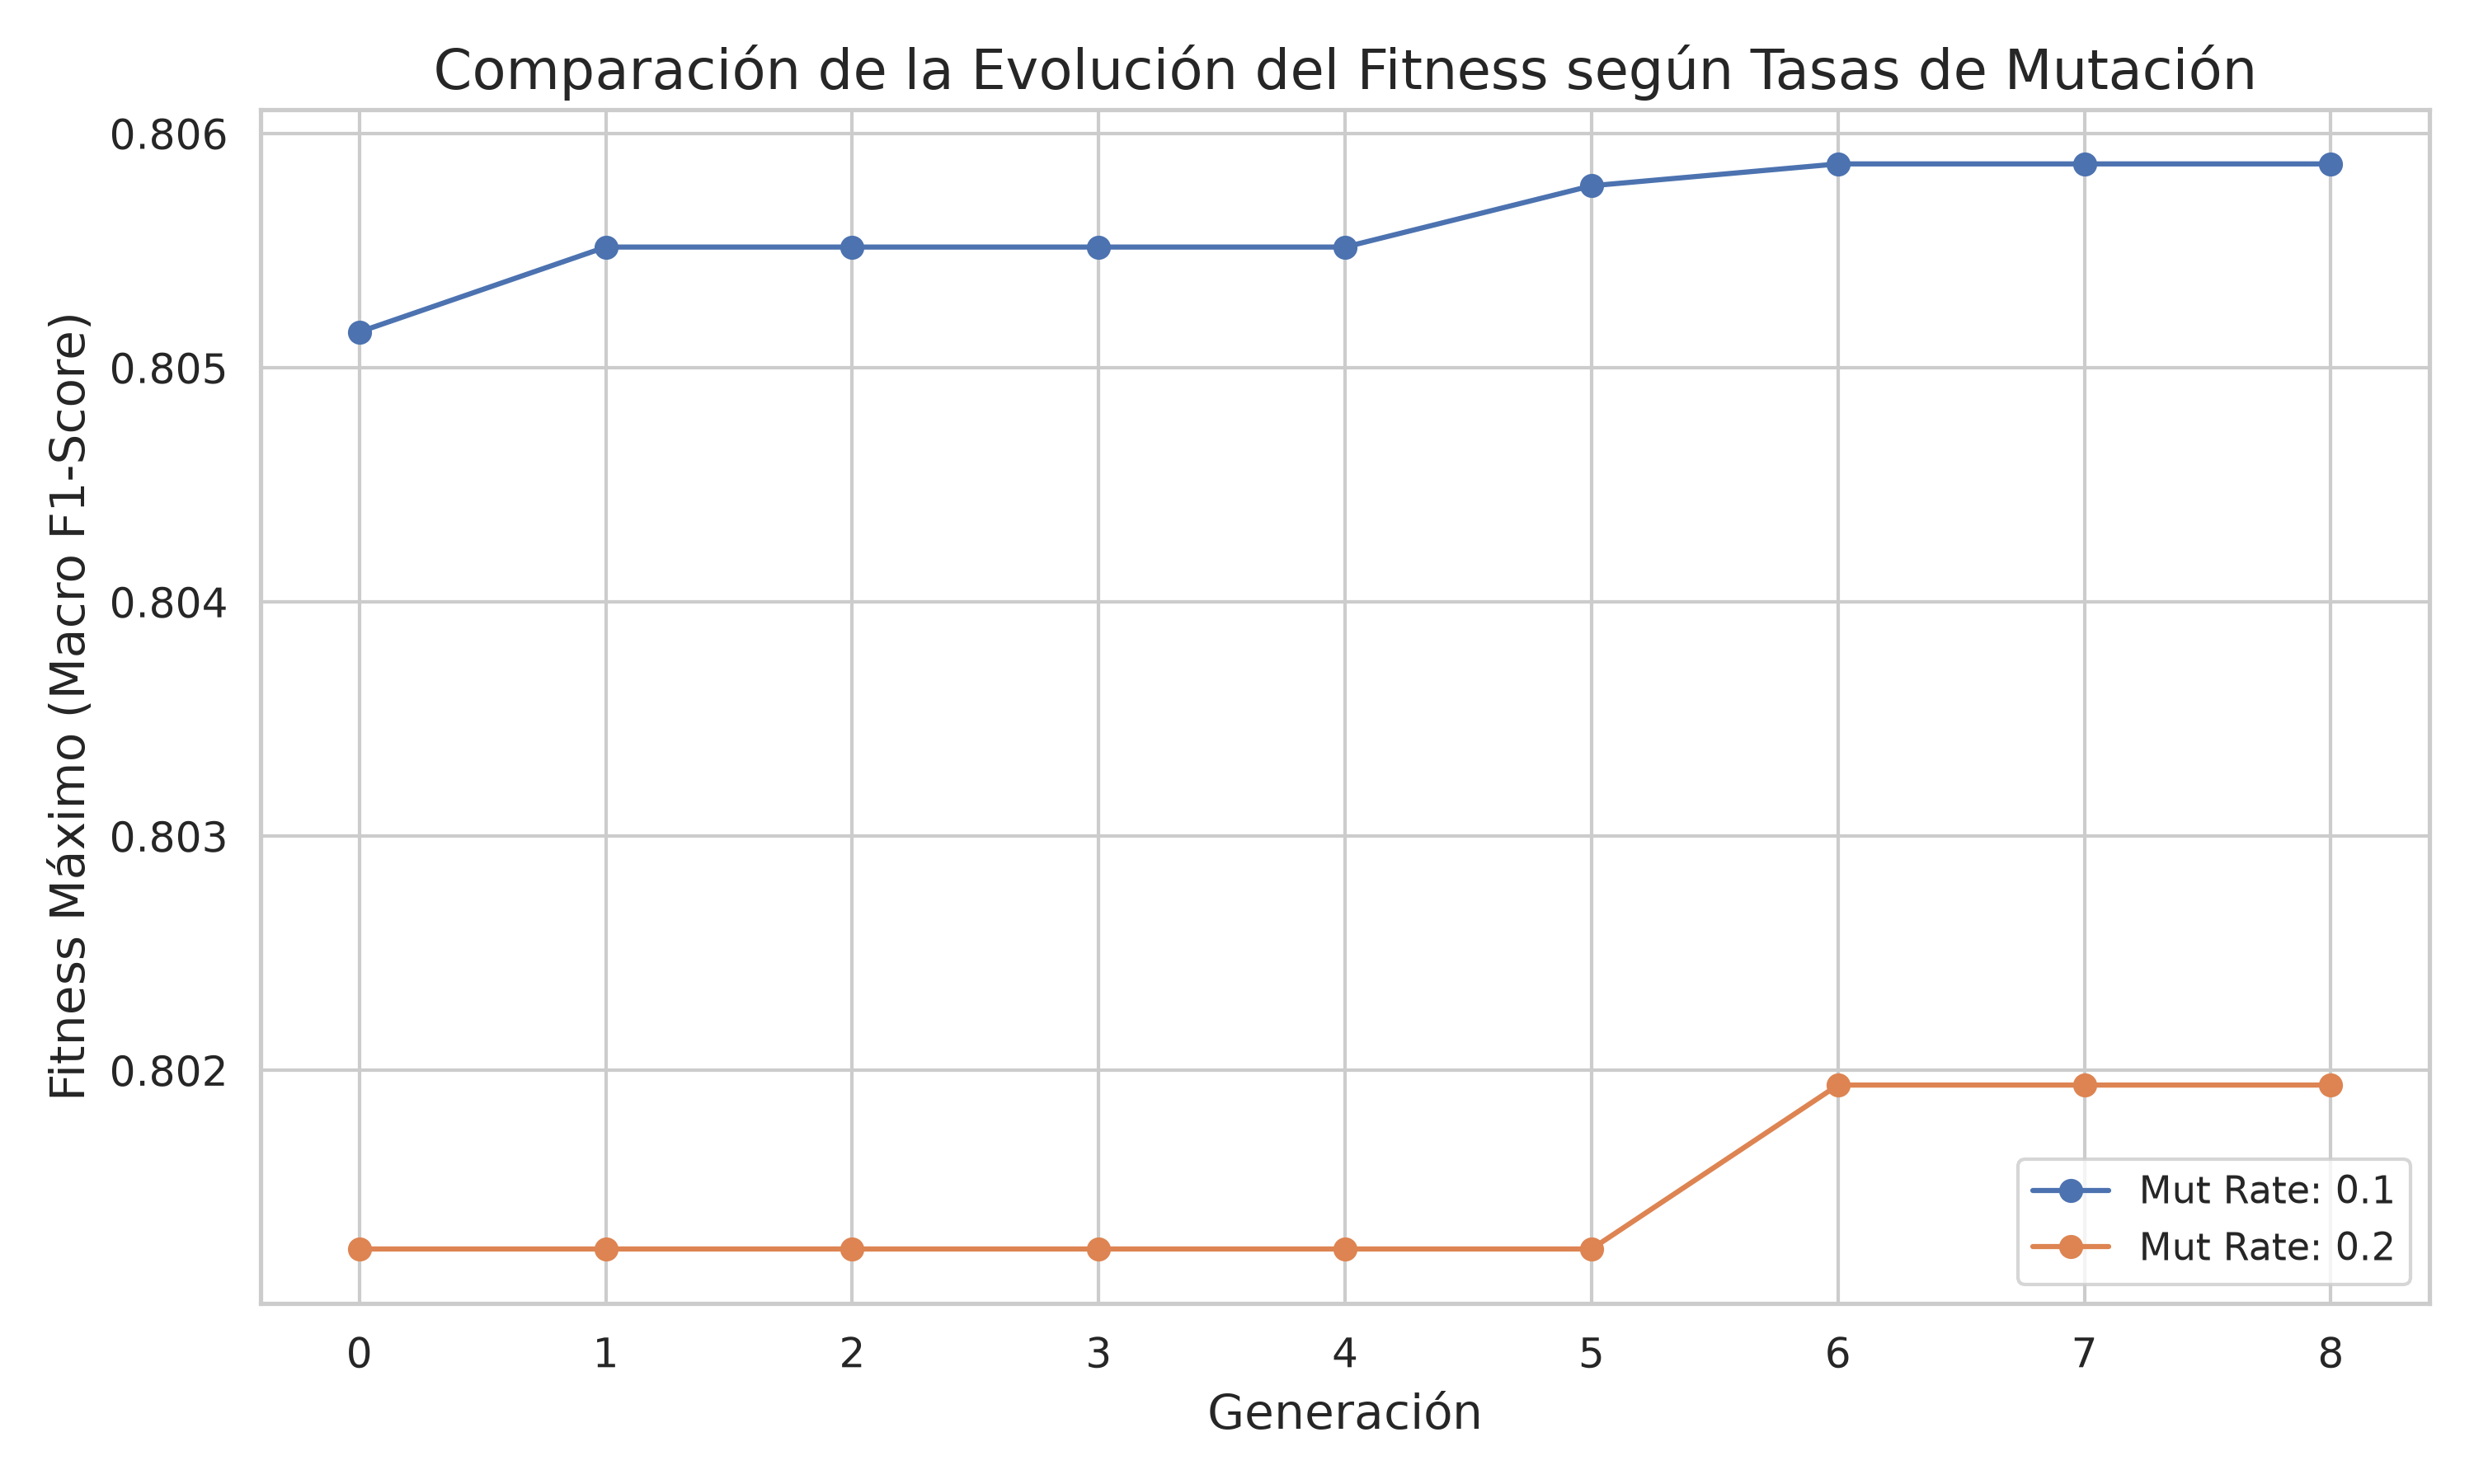
\includegraphics[width=0.92\linewidth]{13_evolucion_fitness_ga.png}
\caption{Evolución de la aptitud durante la optimización de hiperparámetros mediante el algoritmo genético.}
\label{fig:ga-fitness}
\end{figure}

\begin{figure}[htbp]
\centering
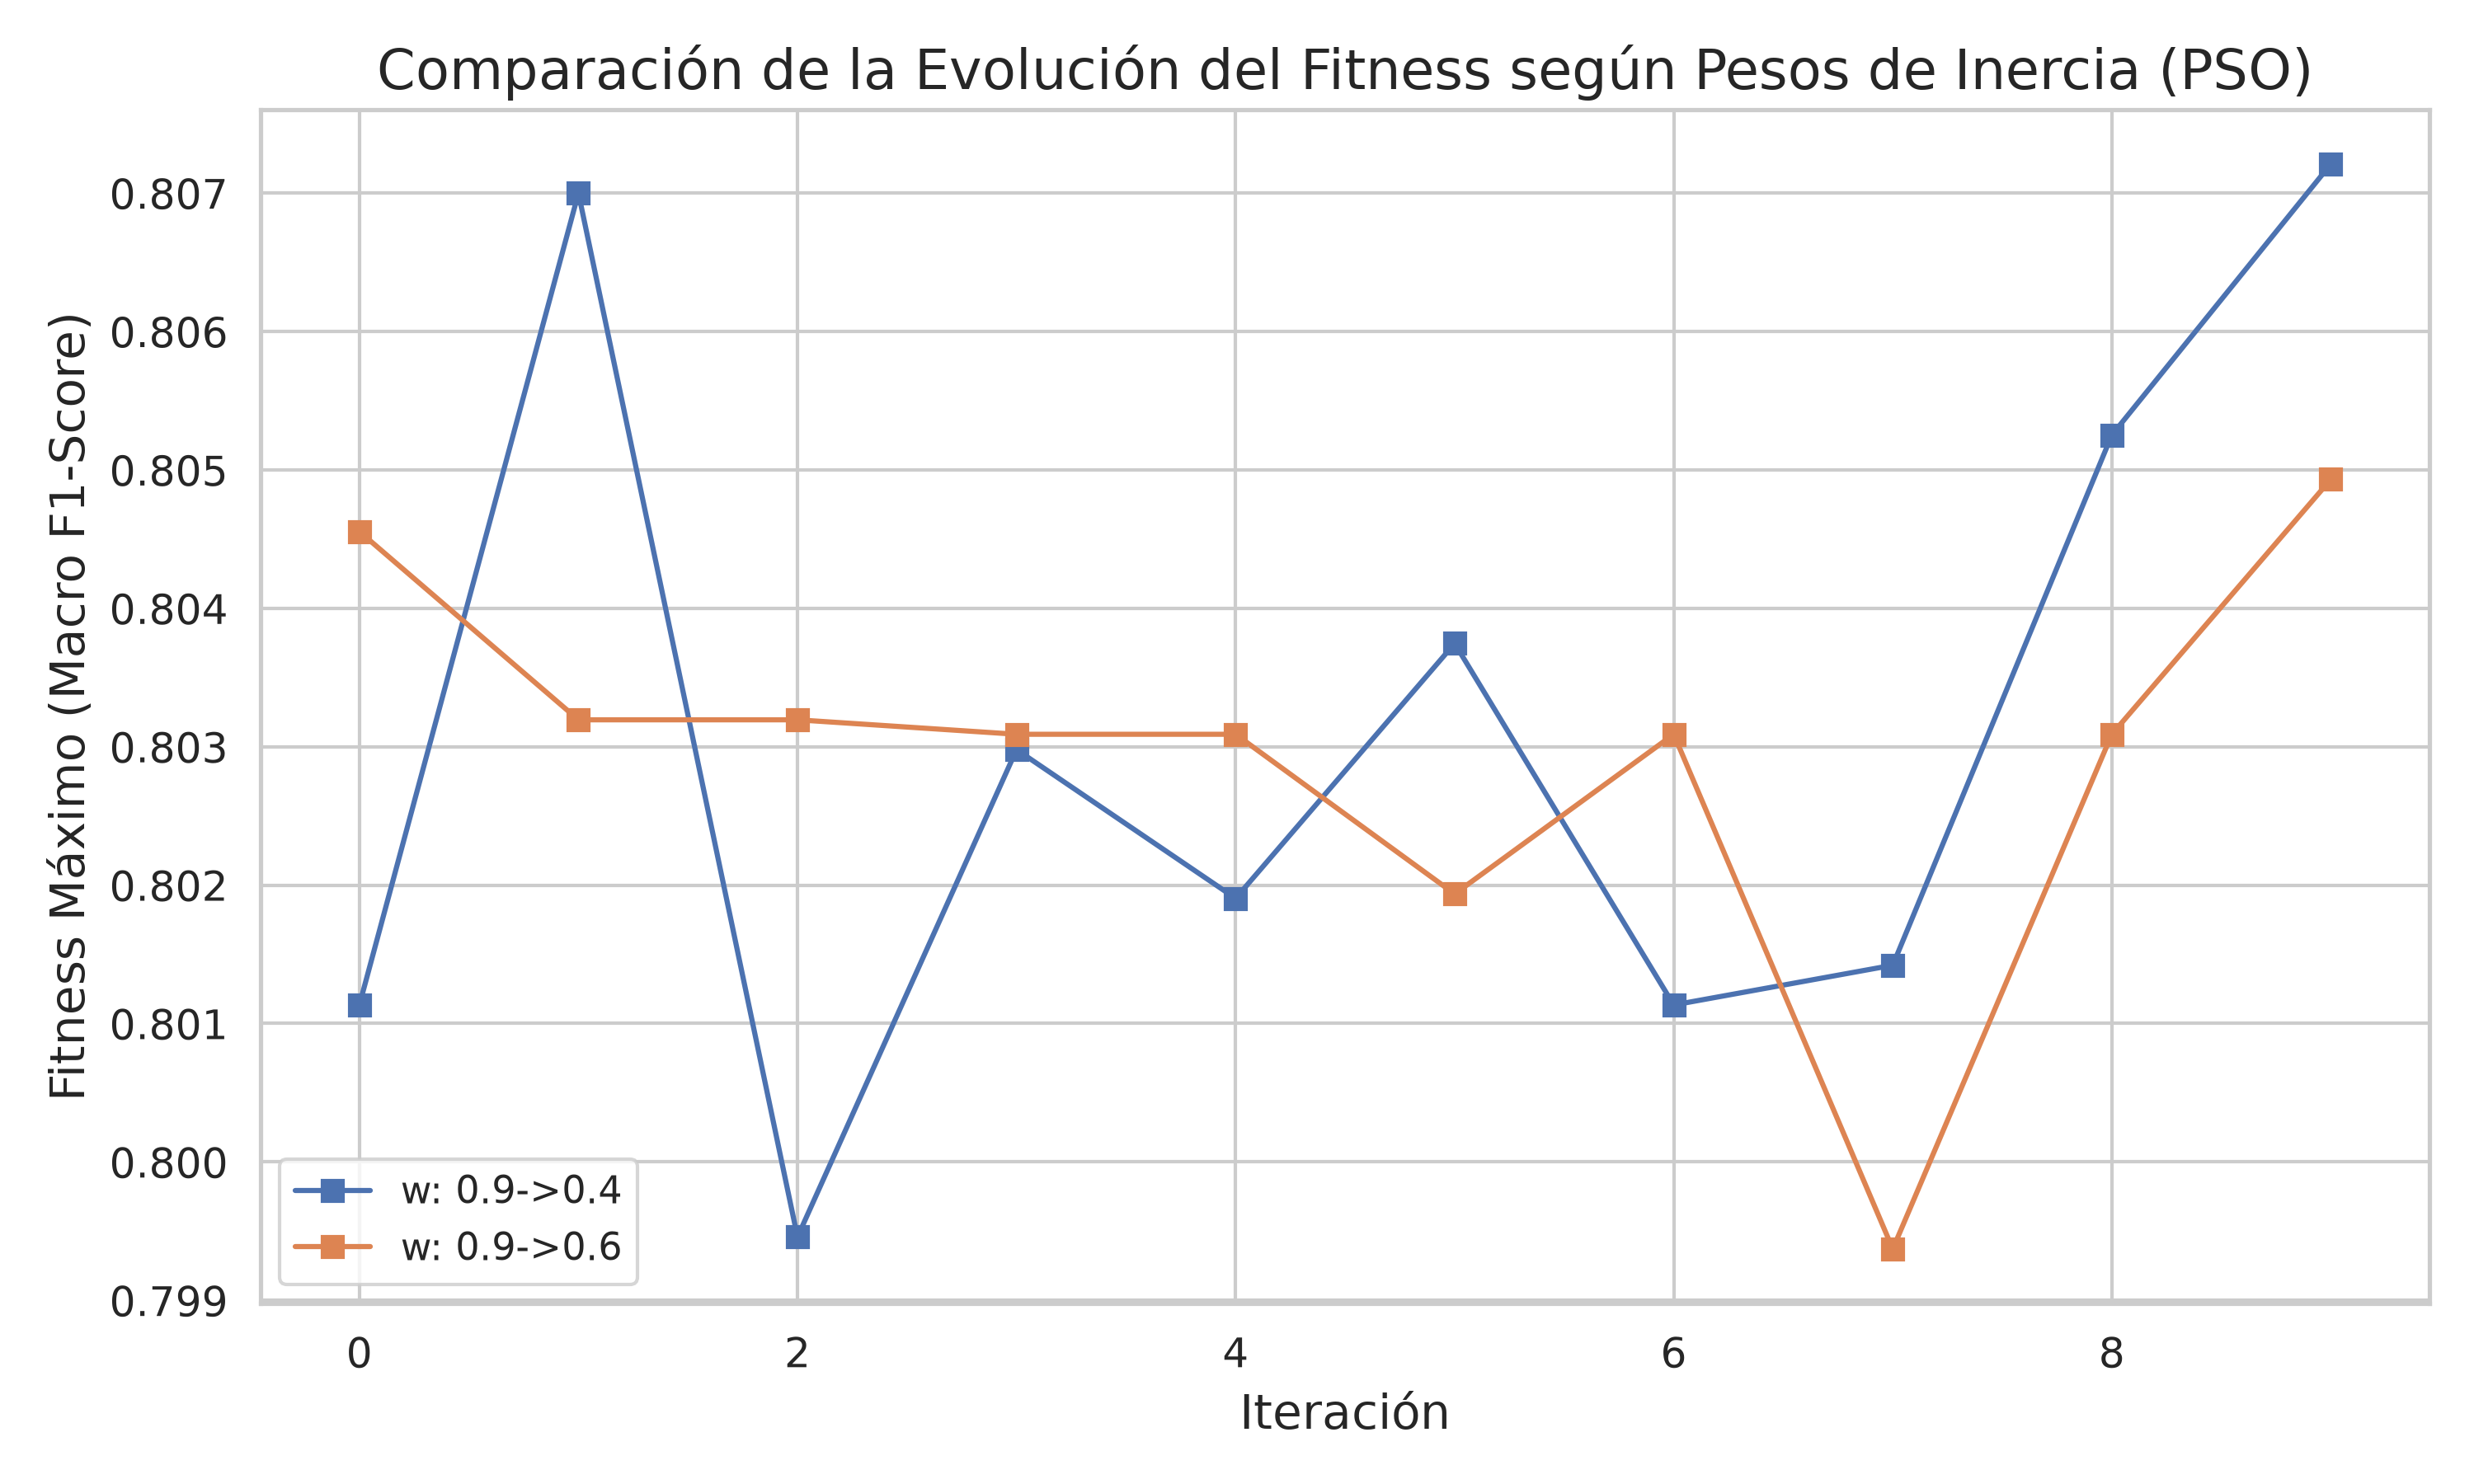
\includegraphics[width=0.92\linewidth]{13_evolucion_fitness_pso.png}
\caption{Evolución de la aptitud durante la optimización de hiperparámetros mediante enjambre de partículas (PSO).}
\label{fig:pso-fitness}
\end{figure}

Las curvas de pérdida y exactitud obtenidas durante el entrenamiento y la validación de los modelos se presentan en la Fig. \ref{fig:curvas-entrenamiento}.

\begin{figure}[htbp]
\centering
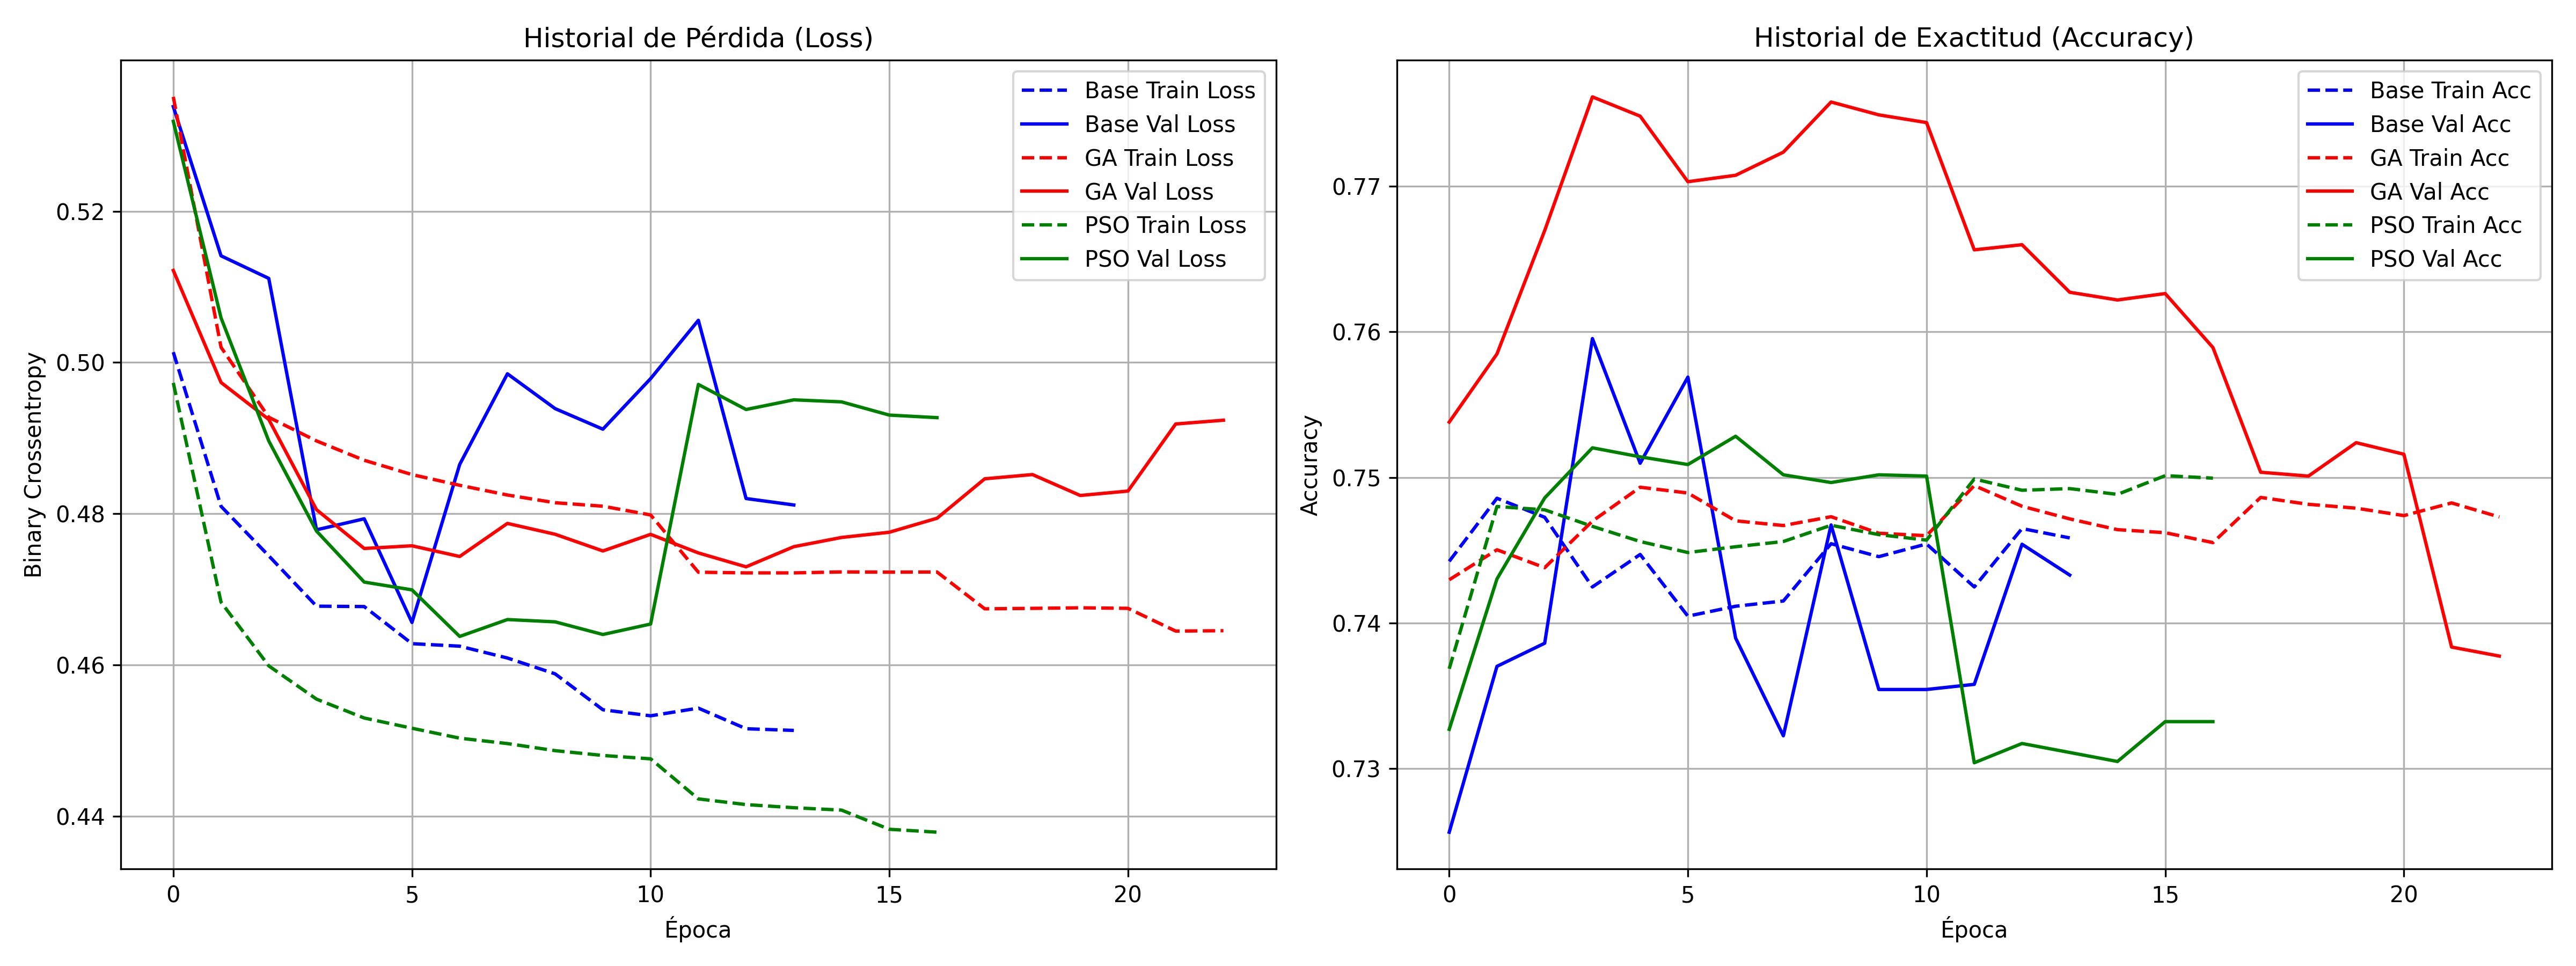
\includegraphics[width=0.95\linewidth]{17_curvas_entrenamiento_comparativas.png}
\caption{Curvas comparativas de pérdida y exactitud durante el entrenamiento y la validación de los tres clasificadores.}
\label{fig:curvas-entrenamiento}
\end{figure}

\section{Resultados y Validación Estadística}
Los tres clasificadores se evaluaron sobre un conjunto de prueba independiente de 11,328 reportes mediante el umbral óptimo de cada modelo. La Tabla \ref{tab:experimentos} resume su rendimiento predictivo y su eficiencia computacional. Dado el severo desbalanceo de clases (93.18\% frente a 6.82\%), la exactitud (\textit{accuracy}) resulta una métrica sesgada si se analiza de forma aislada (un clasificador ingenuo obtendría 93.18\% de exactitud sin capacidad de detección real). Por tanto, el análisis se centra principalmente en el F1-Score macro y la sensibilidad (\textit{recall}) para evaluar de manera justa la discriminación sobre la clase de alto riesgo.


\begin{table*}[htbp]
\caption{Métricas comparativas en el conjunto de prueba}
\label{tab:experimentos}
\centering
\scriptsize
\setlength{\tabcolsep}{4pt}
\begin{tabular}{lccccccccc}
\toprule
\textbf{Modelo} & \textbf{Exactitud} & \textbf{Precisión} & \textbf{Sensibilidad} & \textbf{F1 macro} & \textbf{ROC-AUC} & \textbf{PR-AUC} & \textbf{Log loss} & \textbf{Entrenam. (s)} & \textbf{Latencia (ms)} \\
\midrule
MLP base & 90.78\% & 0.6573 & 0.6897 & 0.6714 & 0.8660 & 0.9877 & 0.4718 & 163.15 & 0.0519 \\
MLP + GA & 90.73\% & 0.6585 & 0.6961 & 0.6745 & 0.8645 & 0.9873 & 0.4692 & 374.52 & 0.0601 \\
MLP + PSO & 90.17\% & 0.6499 & 0.7009 & 0.6702 & 0.8672 & 0.9881 & 0.4704 & 98.74 & 0.0654 \\
\bottomrule
\end{tabular}
\end{table*}

\begin{figure}[htbp]
\centering
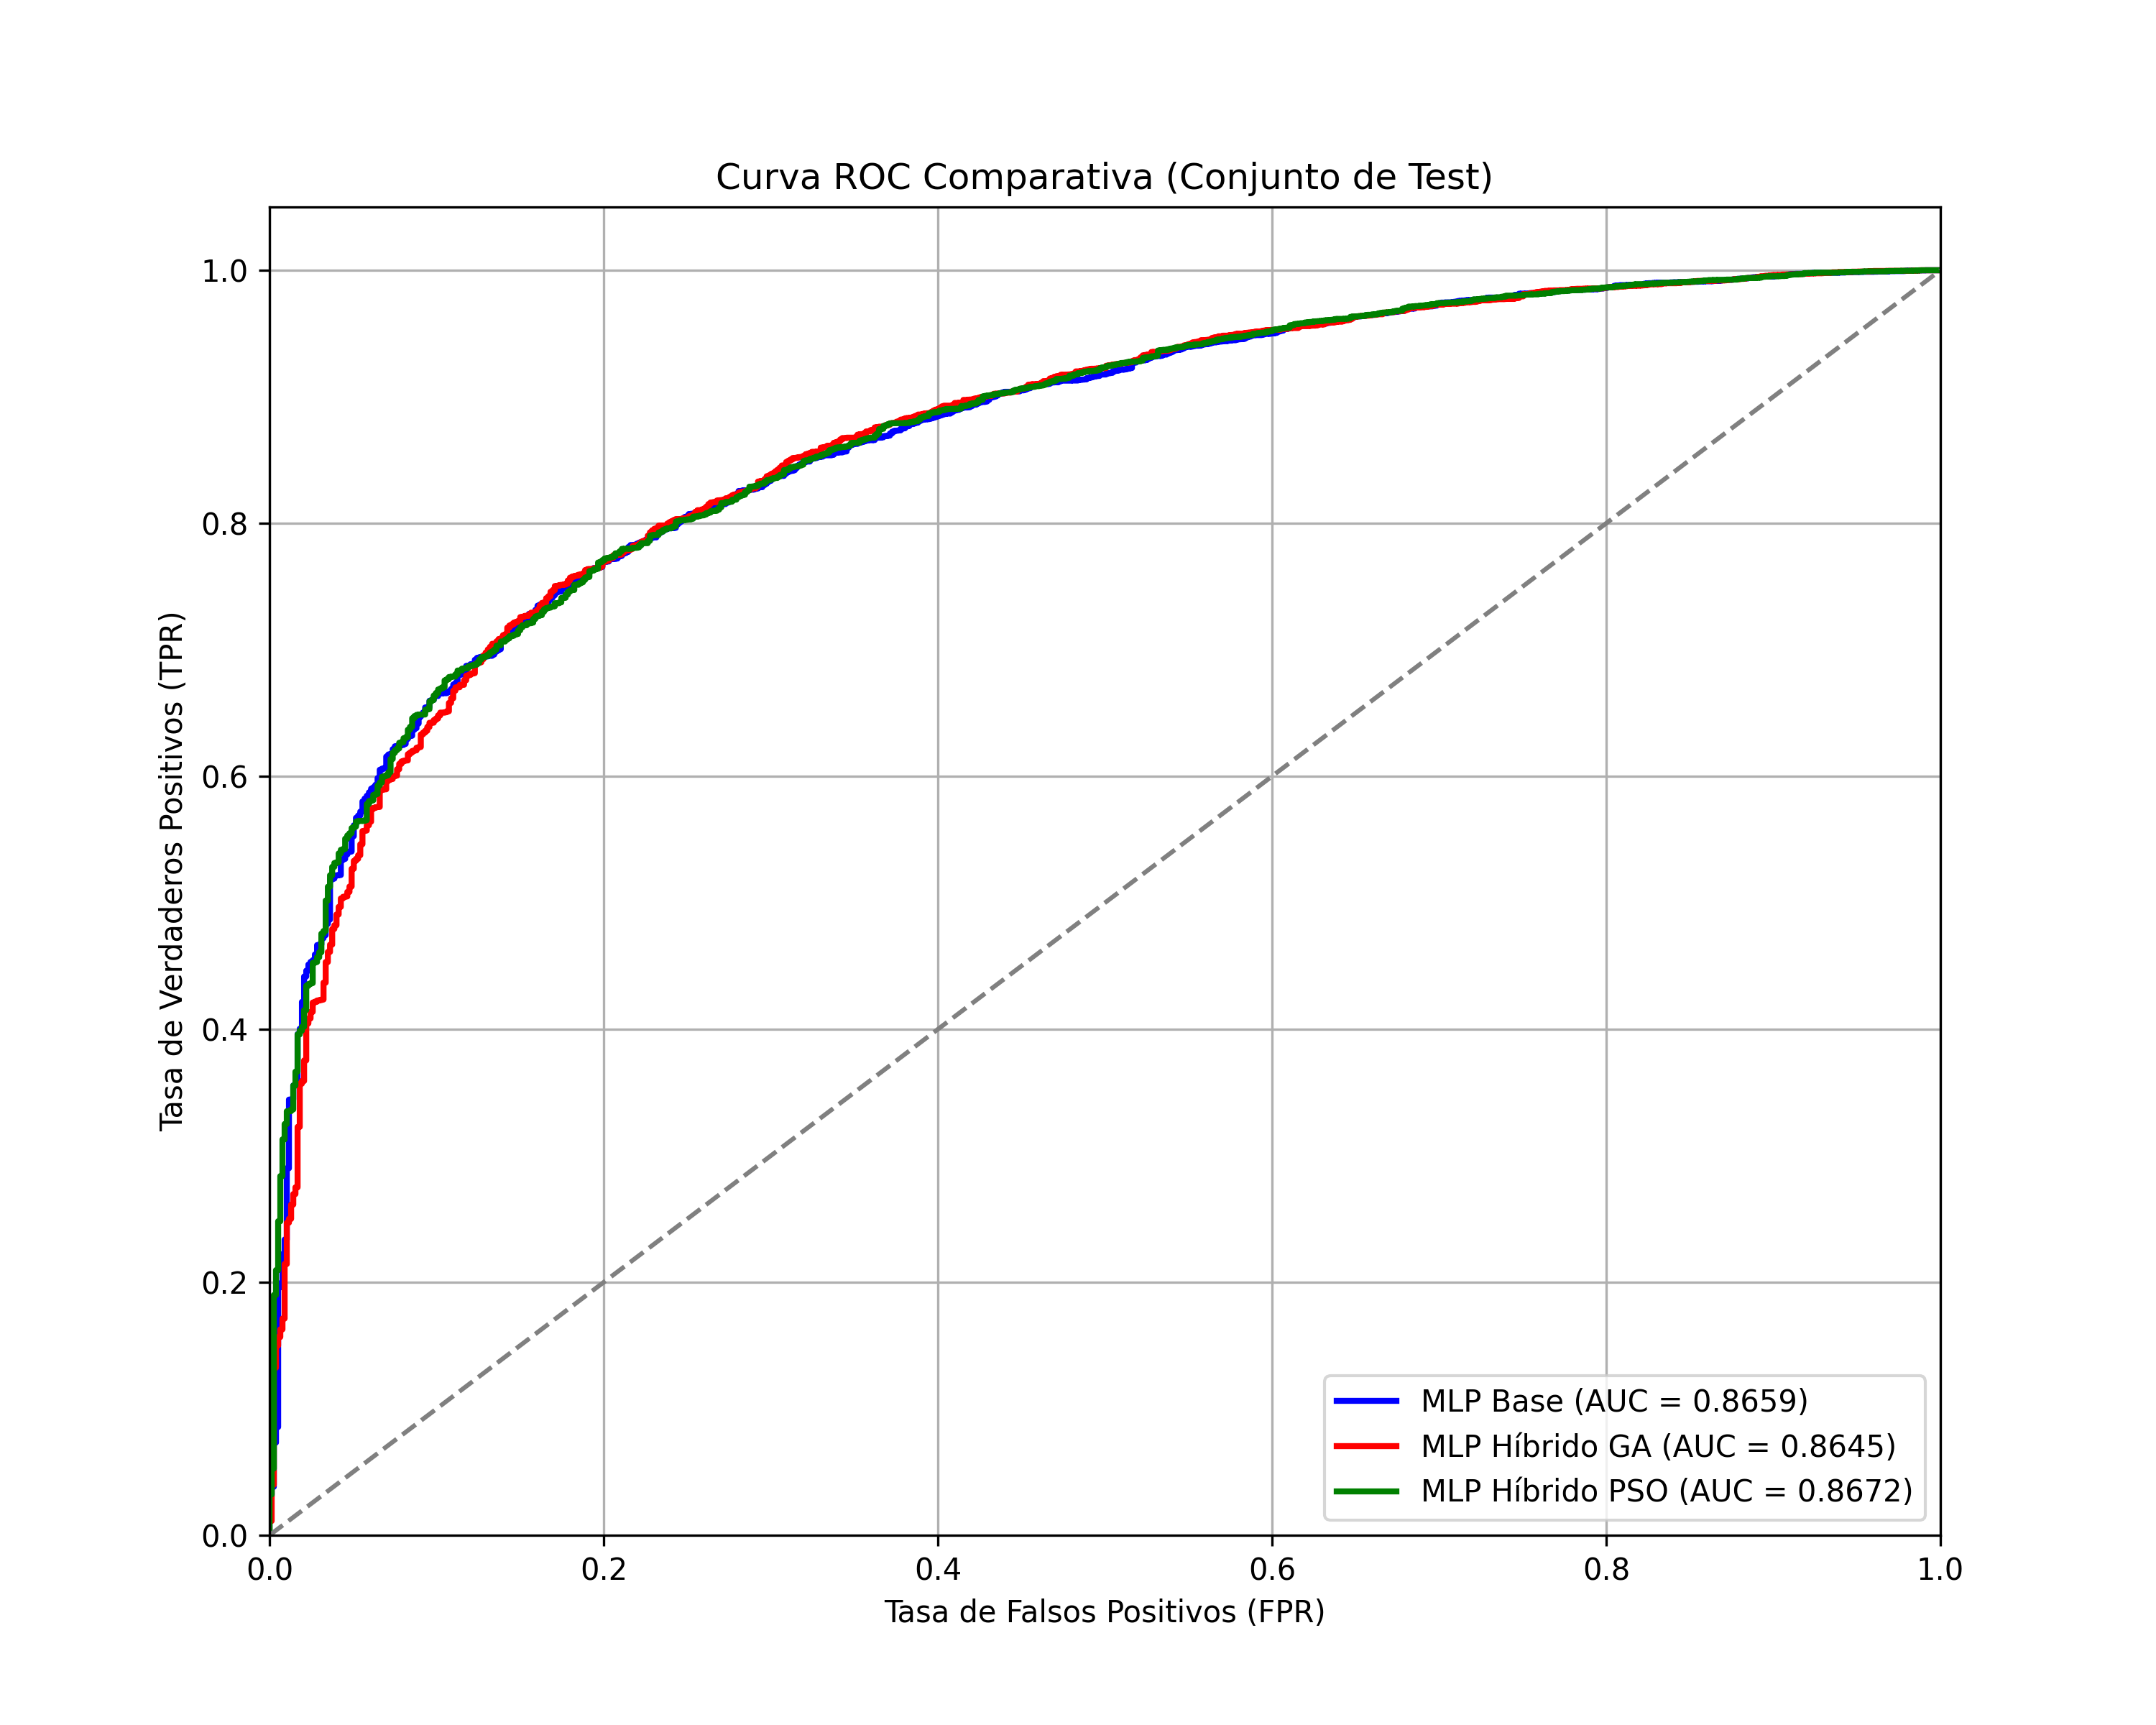
\includegraphics[width=0.95\linewidth]{14_curva_roc_comparativa.png}
\caption{Curvas ROC comparativas obtenidas sobre el conjunto de prueba independiente para los tres modelos entrenados.}
\label{fig:curvas-roc}
\end{figure}

El MLP base obtuvo la mayor exactitud (90.78\%) y la menor latencia de inferencia (0.0519 ms), por lo que ofrece el mejor equilibrio general entre rendimiento y costo computacional. MLP + GA alcanzó el menor \textit{log loss} (0.4692) y el mayor F1 macro (0.6745). Por su parte, MLP + PSO obtuvo la mayor sensibilidad (0.7009), los valores más altos de ROC-AUC (0.8672) y PR-AUC (0.9881), y el menor tiempo de entrenamiento (98.74 s), un 39.48\% inferior al del modelo base. En consecuencia, PSO puede resultar conveniente cuando se prioriza la reducción de falsos negativos y la rapidez de reentrenamiento. Las latencias de inferencia de los tres modelos permanecieron por debajo de 0.07 ms por caso.

\begin{figure}[htbp]
\centering
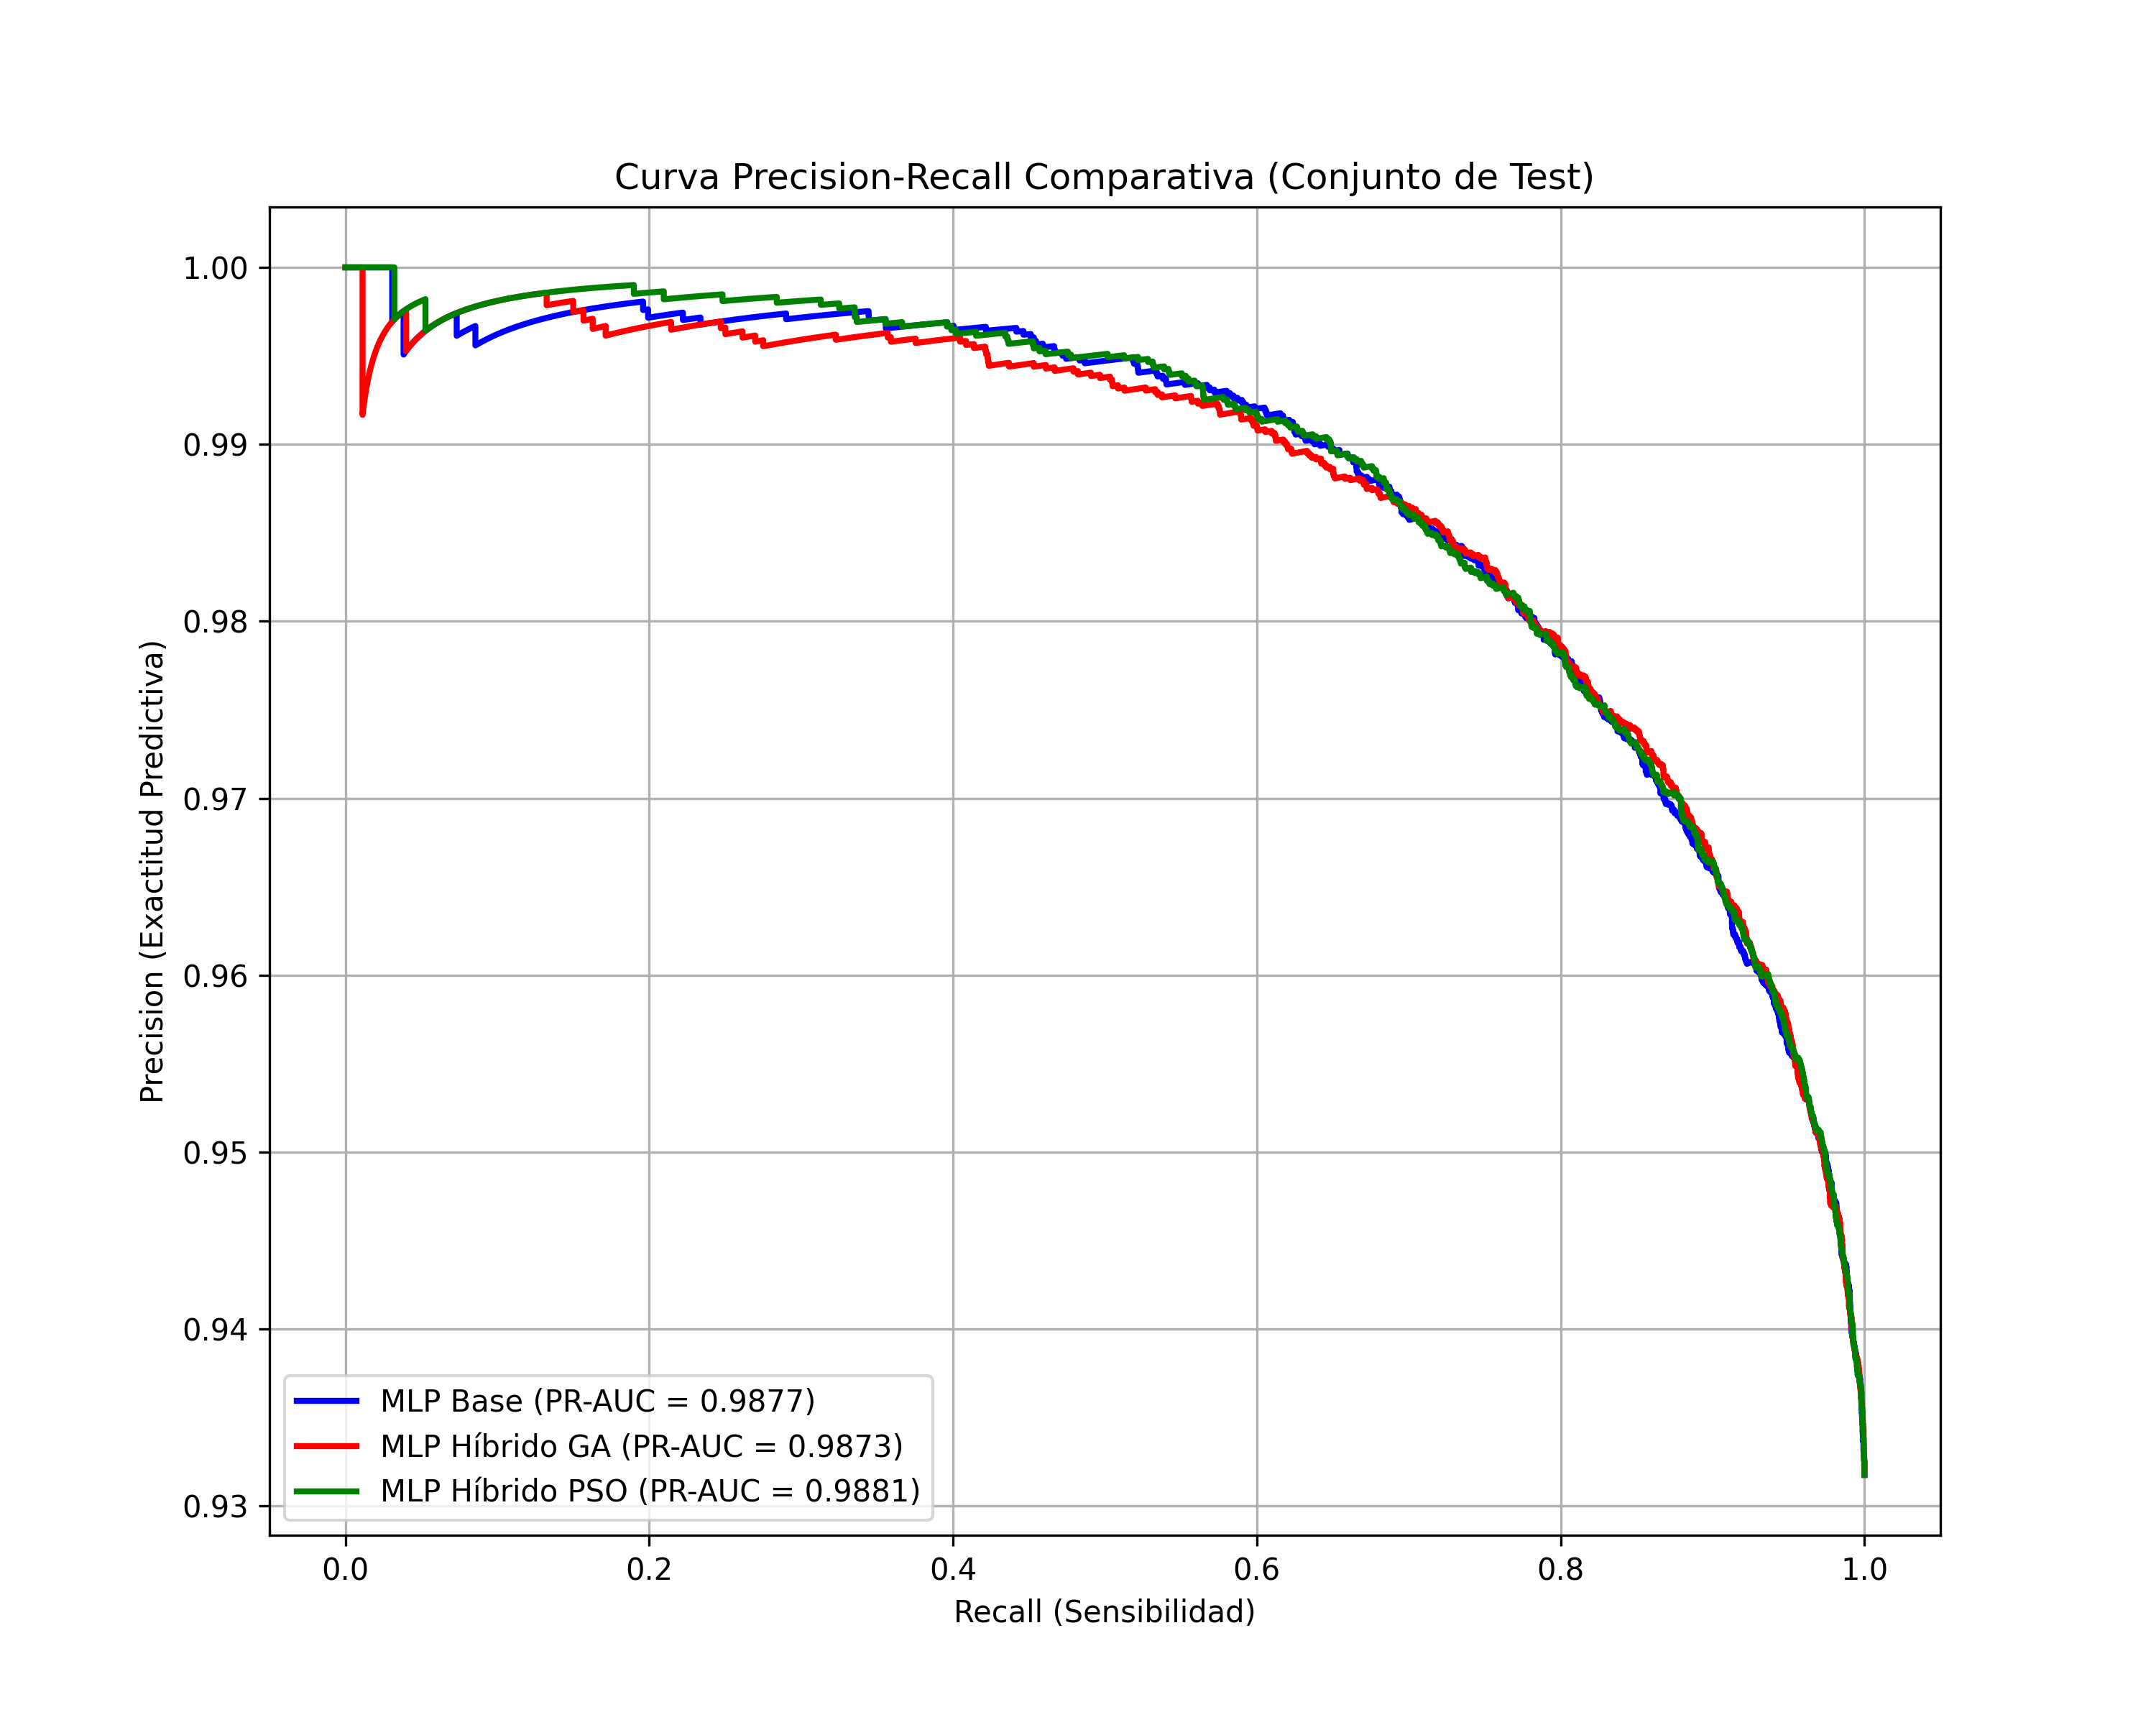
\includegraphics[width=0.95\linewidth]{15_curva_pr_comparativa.png}
\caption{Curvas precisión--sensibilidad comparativas sobre el conjunto de prueba para los tres modelos entrenados.}
\label{fig:curvas-pr}
\end{figure}

Para analizar detalladamente la distribución de aciertos y errores de clasificación, la Fig. \ref{fig:confusion-matrices} expone las matrices de confusión del conjunto de prueba independiente.

\begin{figure}[htbp]
\centering
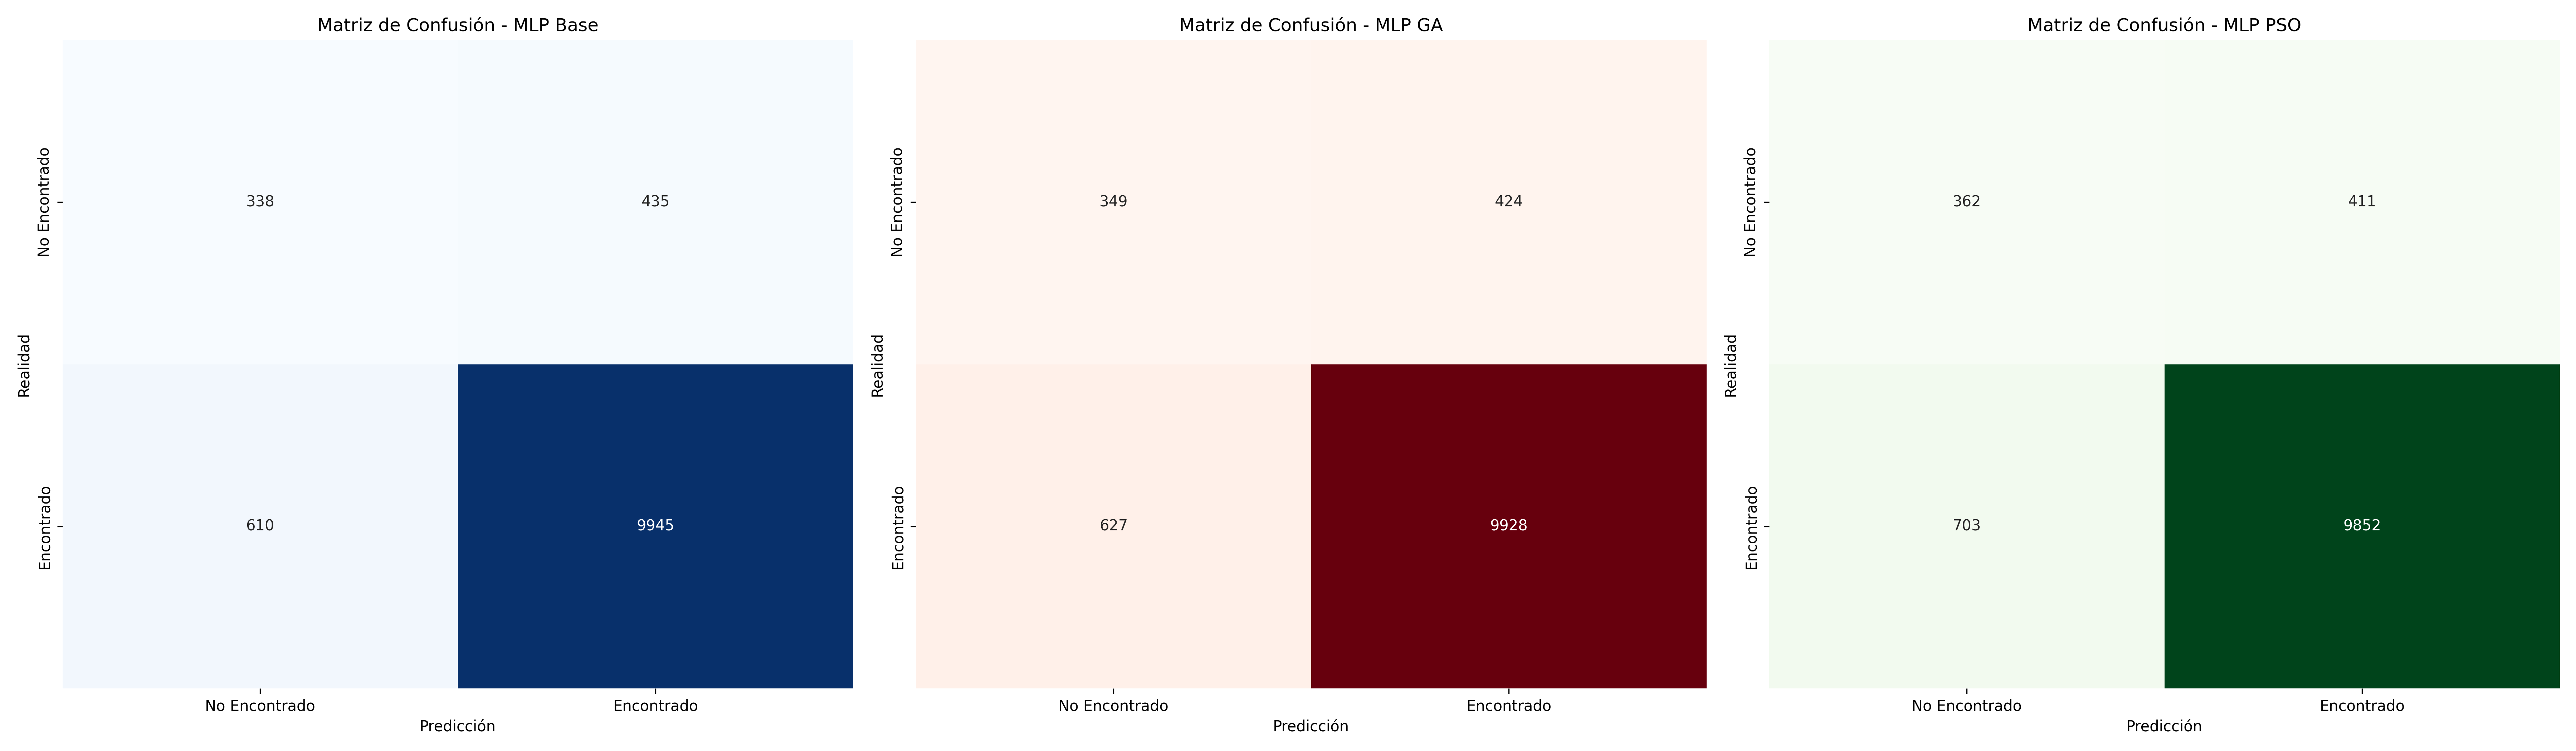
\includegraphics[width=0.95\linewidth]{16_matrices_confusion.png}
\caption{Matrices de confusión comparativas obtenidas sobre el conjunto de prueba independiente para MLP base, MLP + GA y MLP + PSO.}
\label{fig:confusion-matrices}
\end{figure}

Para comparar estadísticamente las predicciones de las arquitecturas, se aplicó la prueba de McNemar descrita en la Ec. \ref{eq:mcnemar}.
\begin{itemize}
    \item \textbf{MLP base frente a MLP + GA:} El estadístico chi-cuadrado fue 0.0838, con un valor $p=0.7723$. Al no rechazarse la hipótesis nula ($p>0.05$), no se encontró evidencia de diferencias significativas entre sus predicciones. En este contexto, el MLP base conserva la ventaja de una menor complejidad computacional.
    \item \textbf{MLP + GA frente a MLP + PSO:} El estadístico chi-cuadrado fue 15.1489, con un valor $p=9.94\times10^{-5}$. La diferencia fue estadísticamente significativa ($p<0.05$), lo que indica que ambas estrategias de optimización producen patrones de error distintos.
\end{itemize}

\section{Discusión y Explicabilidad}
La incorporación de la regularización L2 en el espacio de búsqueda del algoritmo genético contribuyó a controlar la complejidad del modelo. Asimismo, el uso de pesos de clase evitó generar coordenadas geográficas sintéticas, como podría ocurrir con técnicas de interpolación aplicadas durante el remuestreo.

Para facilitar la interpretación y auditoría de las inferencias, se integraron dos niveles de explicabilidad \cite{lundberg2017unified,ribeiro2016why}:
\begin{itemize}
    \item \textbf{SHAP (explicación global):} Estima la contribución general de las características. El análisis destacó principalmente la edad, el sexo, la antigüedad en días, el rango etario y el año de desaparición (Fig. \ref{fig:shap}).
    \item \textbf{LIME (explicación local):} Justifica visualmente cada predicción, mostrando qué atributos aumentan o disminuyen la probabilidad estimada para un caso individual.
\end{itemize}

\begin{figure}[htbp]
\centering
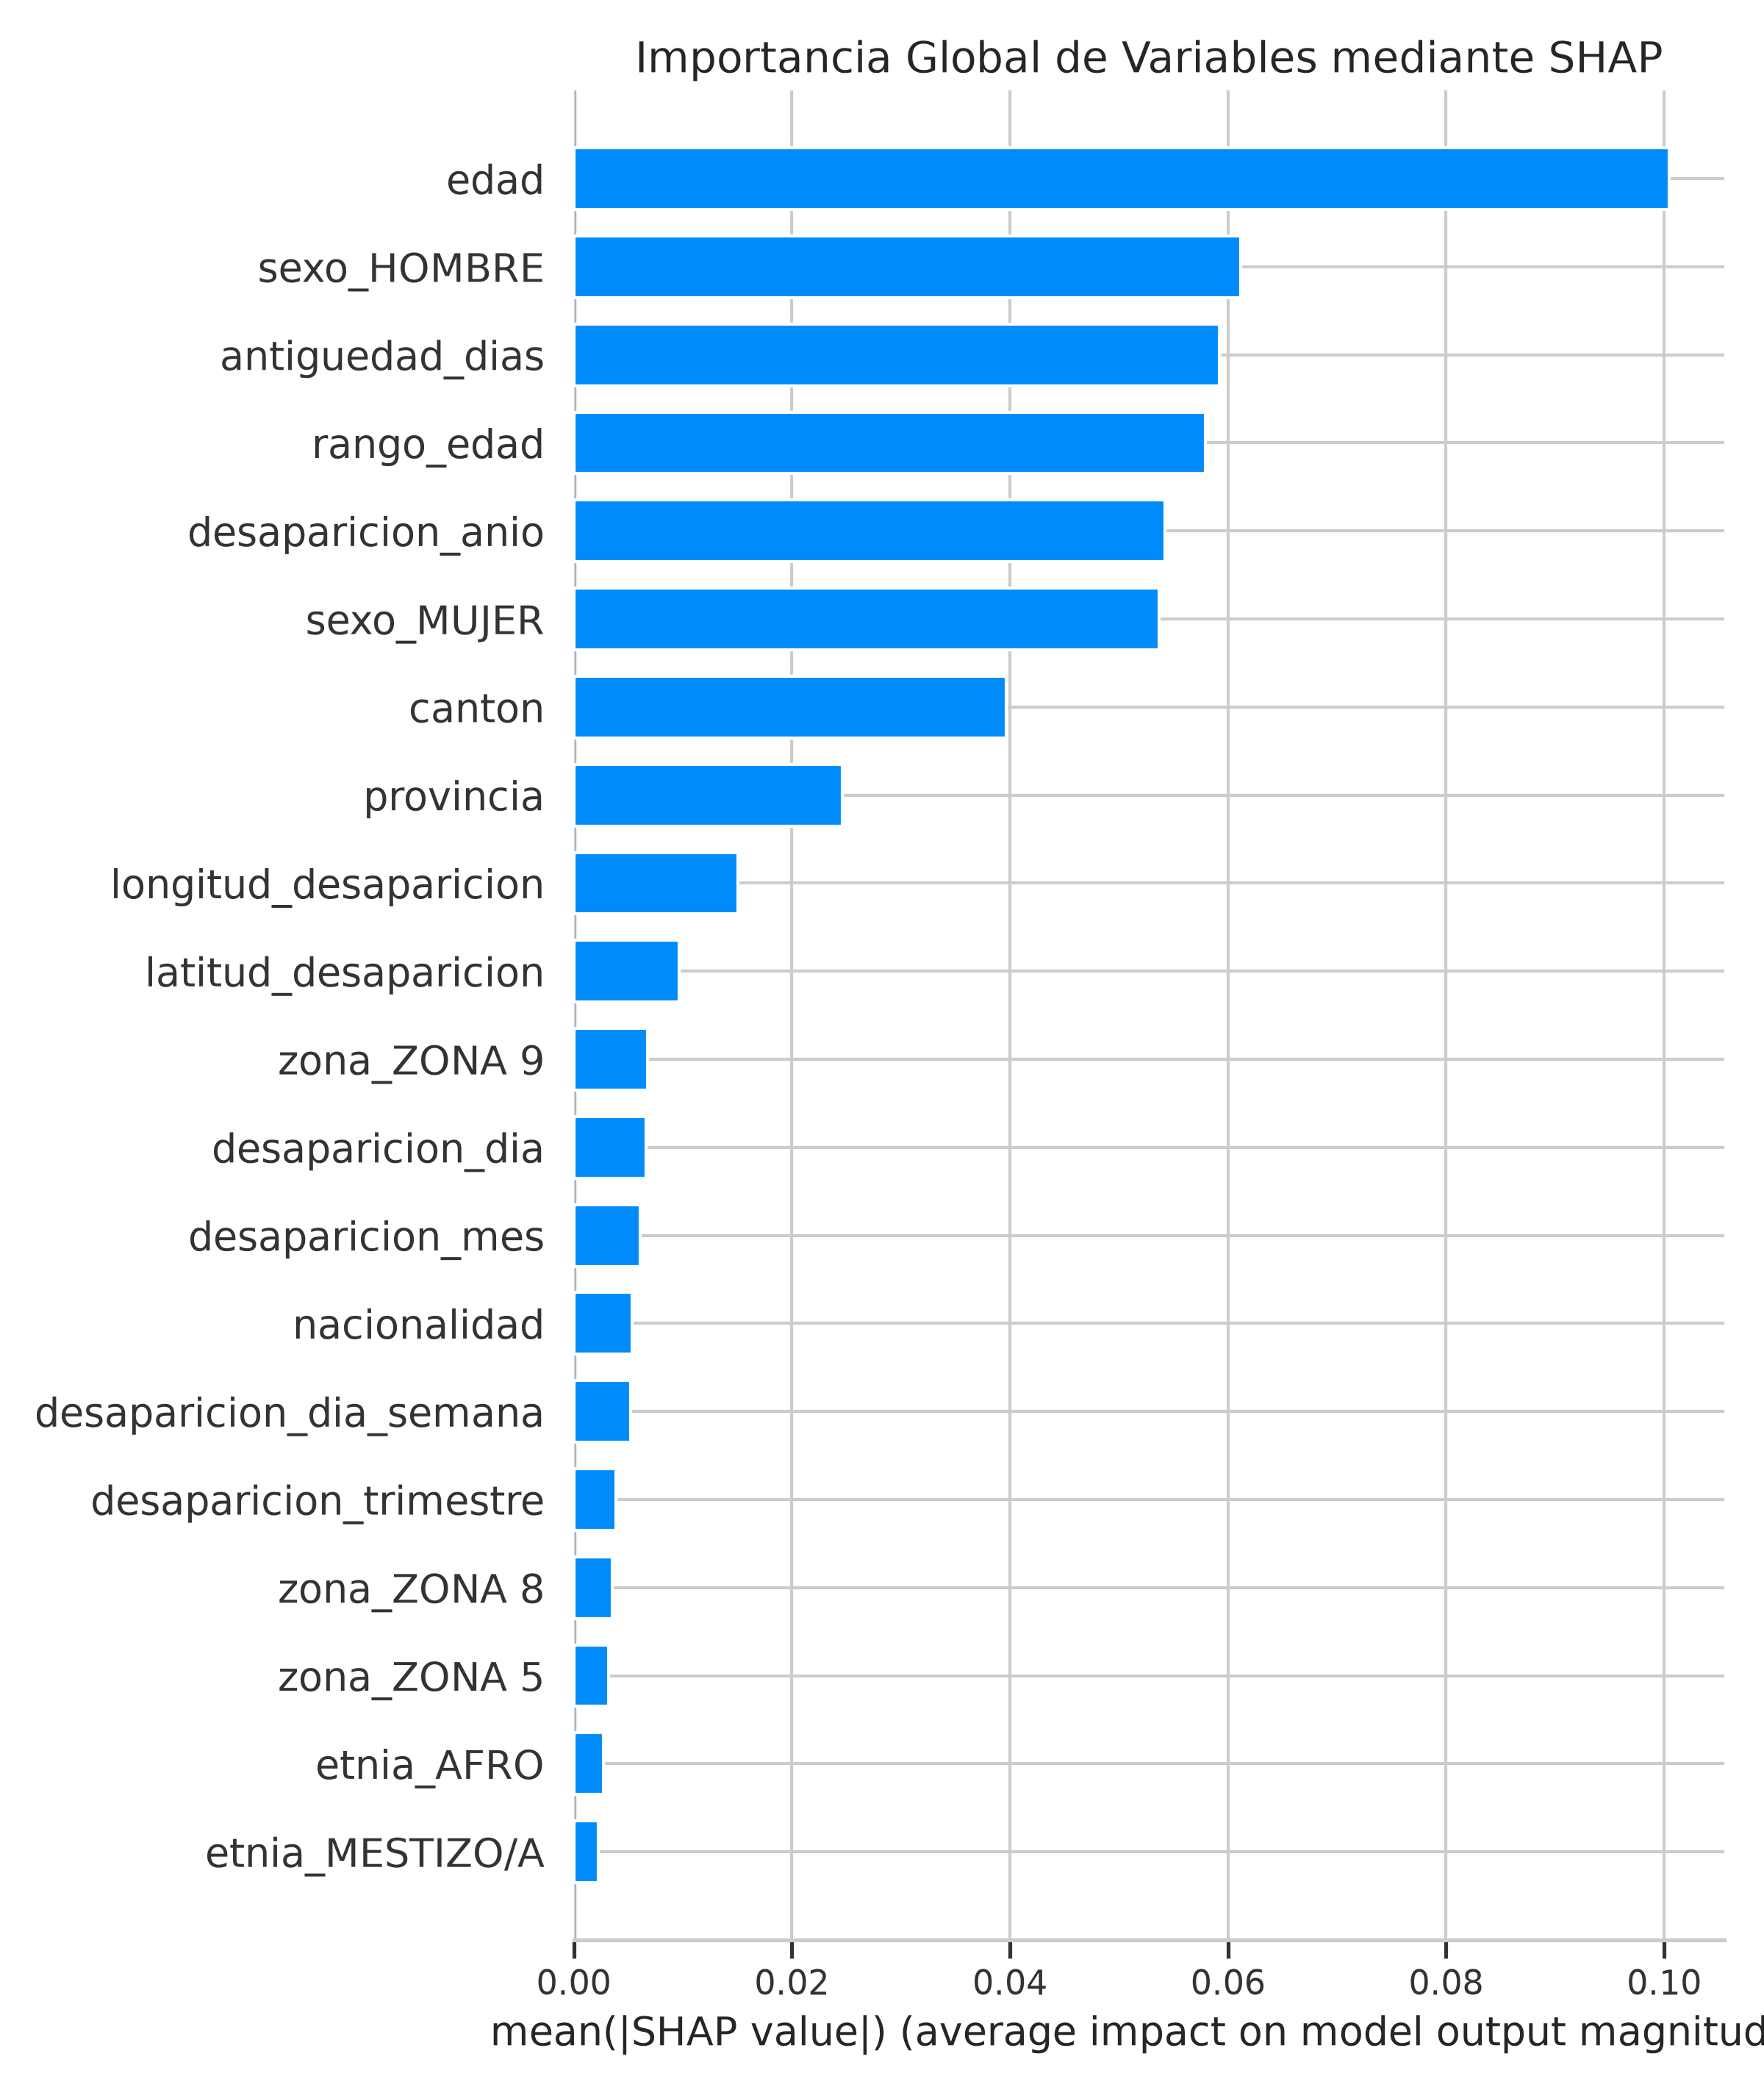
\includegraphics[width=0.92\linewidth]{11_shap_summary_bar.png}
\caption{Importancia global de variables mediante el valor absoluto medio de SHAP para el modelo optimizado.}
\label{fig:shap}
\end{figure}

Un ejemplo del reporte gráfico interactivo proporcionado localmente por LIME se presenta en la Fig. \ref{fig:lime-sample}.

\begin{figure}[htbp]
\centering
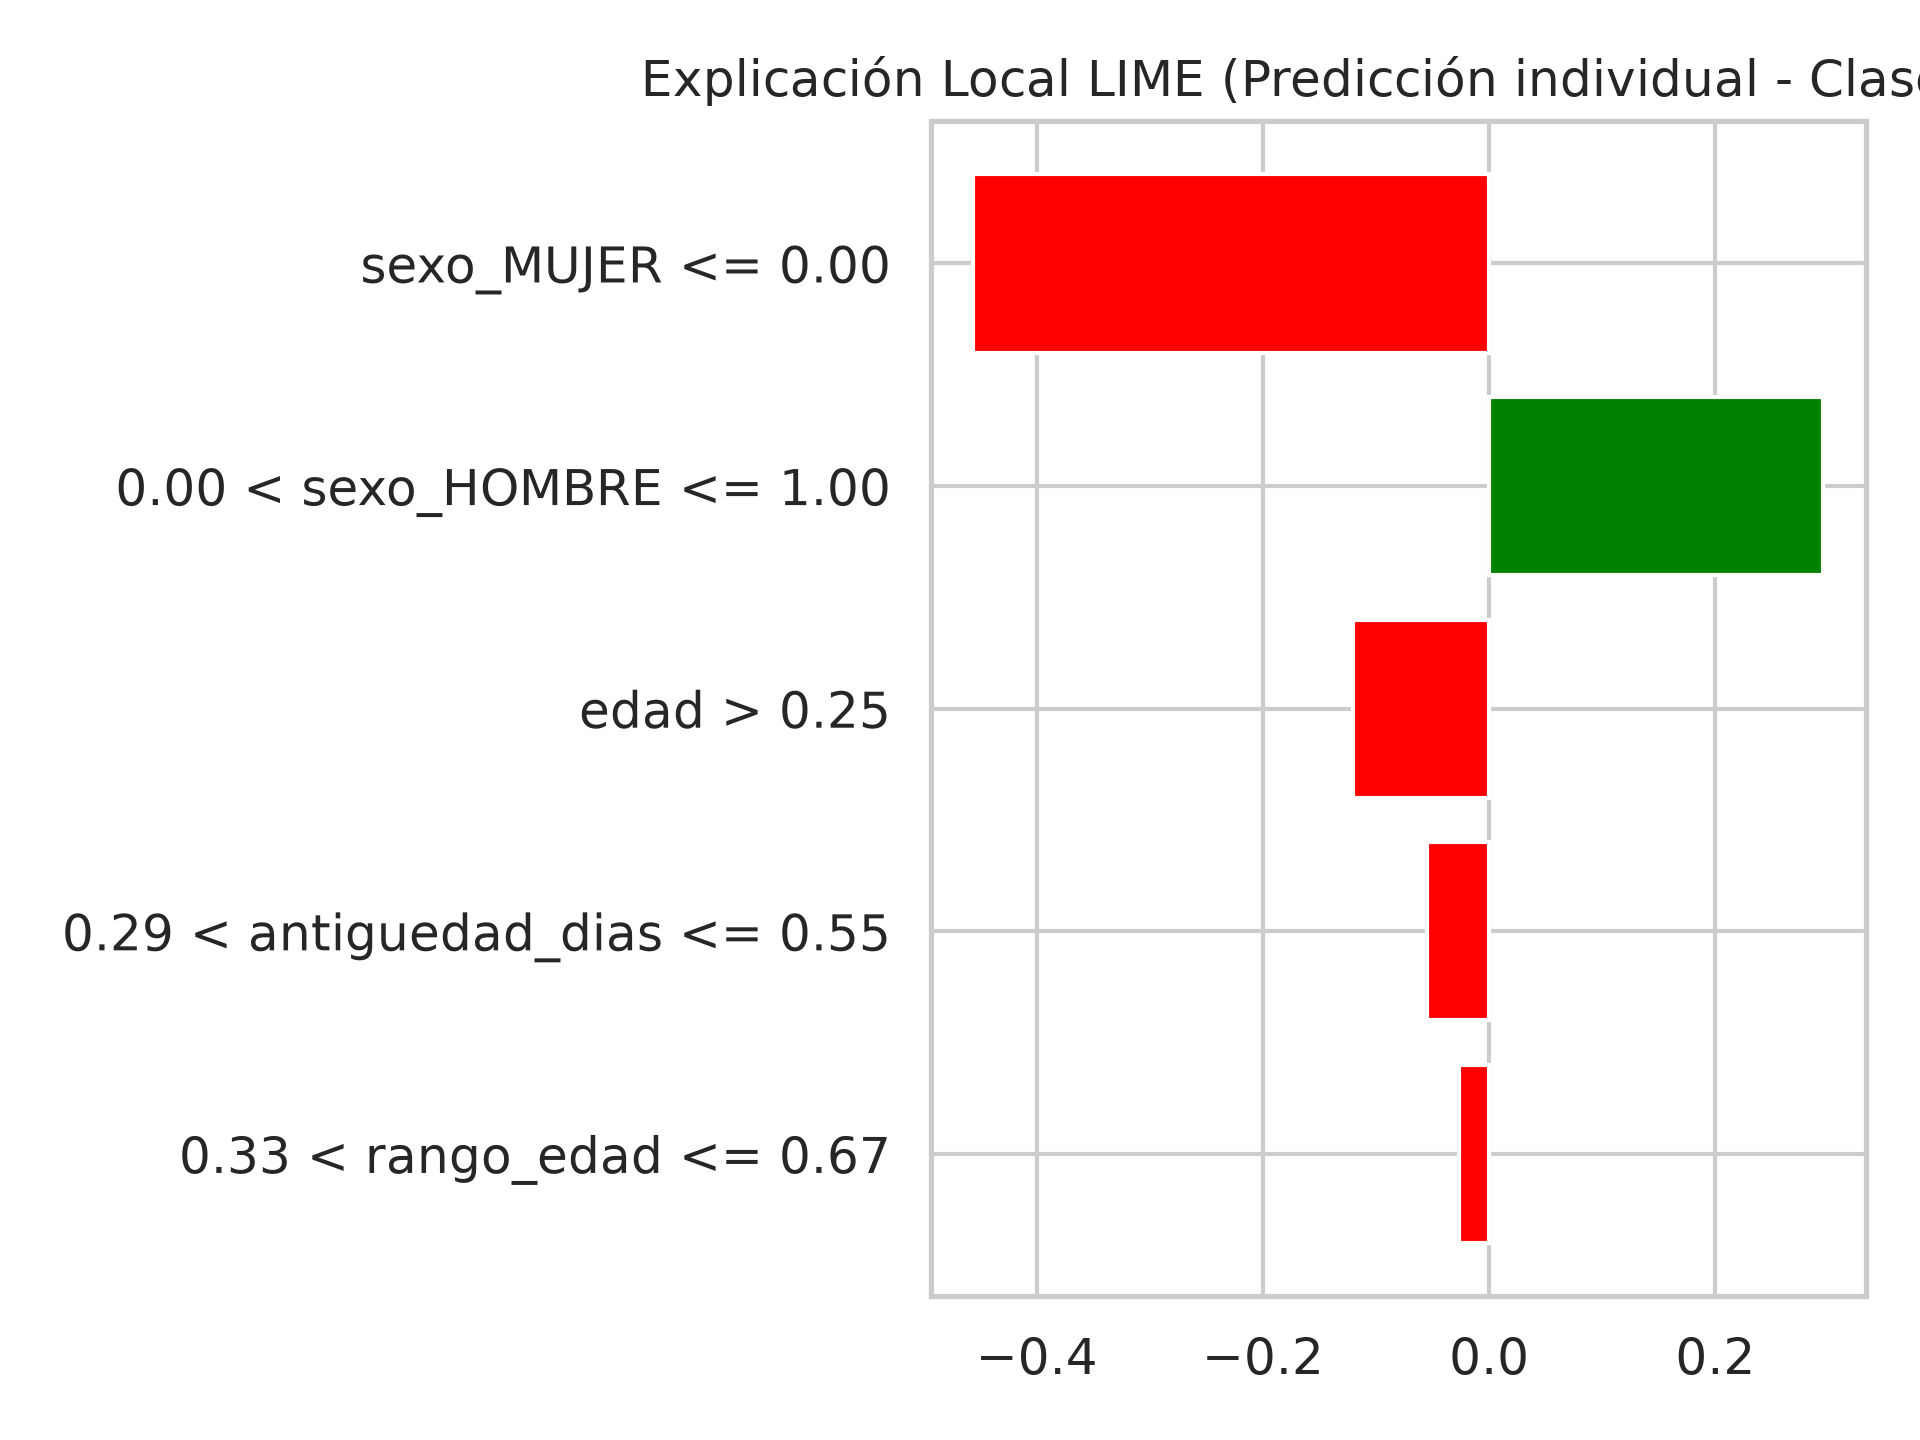
\includegraphics[width=0.95\linewidth]{19_lime_explanation_sample.png}
\caption{Ejemplo de explicación local interactiva individual generada por LIME en la plataforma web Streamlit.}
\label{fig:lime-sample}
\end{figure}

\section{Conclusiones}
En este trabajo se diseñó y validó un pipeline predictivo basado en perceptrones multicapa (MLP) para modelar la localización de personas desaparecidas en Ecuador. A través de la prueba estadística de McNemar, se demostró que no existen diferencias predictivas estadísticamente significativas ($p = 0.7723$) entre el MLP base y la variante optimizada mediante algoritmos genéticos (MLP + GA). Esto consagra al modelo MLP base como la alternativa más eficiente para su despliegue general, al combinar una menor complejidad de desarrollo, la mayor exactitud global ($90.78\%$) y una latencia de inferencia ultra-baja ($0.0519$ ms).

Por otro lado, el acoplamiento MLP + PSO demostró ser una alternativa especializada altamente competitiva, logrando la mayor sensibilidad o \textit{recall} ($70.09\%$) y las áreas bajo la curva más robustas (ROC-AUC de $0.8672$ y PR-AUC de $0.9881$), junto a una reducción del $39.48\%$ en el tiempo de entrenamiento frente a la línea base. Esto la convierte en la opción idónea para despliegues policiales críticos donde la prioridad absoluta sea minimizar los falsos negativos y agilizar la velocidad de reentrenamiento periódico.

La incorporación de explicabilidad local (LIME) y global (SHAP) dentro de la plataforma interactiva de Streamlit cierra la brecha entre los modelos de caja negra y la toma de decisiones operativas de la Policía Nacional. Como trabajo futuro, se plantea el desarrollo de ensambles de modelos híbridos y la incorporación de variables georreferenciadas de sistemas de información geográfica (SIG) en tiempo real para enriquecer la precisión espacial en el ``día cero'' de la denuncia.

\section*{Agradecimientos}
Los autores agradecen el acompañamiento académico del Mgs. Marco Javier Castelo Cabay, profesor de asignatura, durante el desarrollo de la investigación.

\IEEEtriggeratref{5}
\begin{thebibliography}{00}
\bibitem{biehal2003lost} N. Biehal, F. Mitchell, and J. Wade, \emph{Lost from View: Missing Persons in the UK}. Bristol, UK: Policy Press, 2003.
\bibitem{espinoza2025predictive} M. A. Espinoza-Mina and A. M. Colina Vargas, ``Predictive analysis of missing persons in Ecuador (2014--2024),'' in \emph{CEUR Workshop Proceedings}, vol. 4055, pp. 197--210, 2025.
\bibitem{kaufman2012leakage} S. Kaufman, S. Rosset, C. Perlich, and O. Stitelman, ``Leakage in data mining: Formulation, detection, and avoidance,'' \emph{ACM Transactions on Knowledge Discovery from Data}, vol. 6, no. 4, pp. 1--21, 2012.
\bibitem{lundberg2017unified} S. M. Lundberg and S.-I. Lee, ``A unified approach to interpreting model predictions,'' in \emph{Advances in Neural Information Processing Systems}, vol. 30, 2017.
\bibitem{phoenix2022police} J. Phoenix and B. Francis, ``Police risk assessment and case outcomes in missing person investigations,'' \emph{The Police Journal}, vol. 96, pp. 1--21, 2022.
\bibitem{quinga2025data} P. Quinga, E. Jara, F. Cela, C. Coba, A. Pilco, and V. Moya, ``Data analysis of missing people in Ecuador,'' in \emph{Proc. LACCEI Int. Multi-Conf. Engineering, Education and Technology}, vol. 1, no. 12, 2025.
\bibitem{ribeiro2016why} M. T. Ribeiro, S. Singh, and C. Guestrin, ``Why should I trust you?: Explaining the predictions of any classifier,'' in \emph{Proceedings of the 22nd ACM SIGKDD International Conference on Knowledge Discovery and Data Mining}, 2016, pp. 1135--1144.
\bibitem{ruizrizzo2022predicting} A. L. Ruiz-Rizzo, M. E. Archila-Mel\'{e}ndez, and J. J. F. Gonz\'{a}lez Veloza, ``Predicting the probability of finding missing older adults based on machine learning,'' \emph{Journal of Computational Social Science}, vol. 5, no. 2, pp. 1303--1321, 2022.
\bibitem{sidebottom2025can} A. Sidebottom and T. Davies, ``Can harm be predicted? On the development and validation of a statistical model for predicting harm in missing person incidents,'' \emph{Policing and Society}, vol. 35, no. 9, pp. 1173--1190, 2025.
\bibitem{tansill2026when} G. Tansill, T. Cole, A. Barbin, and S. Hambidge, ``When children go missing: Identifying risk factors to predict repeat incidents,'' \emph{Journal of Criminal Psychology}, vol. 16, no. 3, pp. 417--432, 2026.
\end{thebibliography}

\end{document}